\documentclass[14pt,handout,utf8]{beamer}
%\setlength{\paperwidth}{297mm}
%\setlength{\paperheight}{210mm}
%\usepackage[scale=0.78,size=a1]{beamerposter}
\usepackage[scale=1.0,size=a4,orientation=portrait]{beamerposter}
%\setlength{\topmargin}{20mm}
\setbeamersize{text margin left=10mm,text margin right=10mm}

\usepackage{cmap}
\usepackage[T1,T2A]{fontenc}
\usefonttheme[onlymath]{serif}
\usepackage{paratype}
\usepackage{latexsym}
%\usepackage{fancybox}
\usepackage{fouriernc}
\usepackage{mathtools}

\usepackage{scrextend}
\changefontsizes{16pt}

%\usepackage{caption}
\setbeamertemplate{caption}[numbered]
\setbeamertemplate{caption label separator}[endash]
%\addtobeamertemplate{navigation symbols}{}{ \hspace{1em}  \usebeamerfont{footline}  {\normalsize \insertframenumber / \inserttotalframenumber}}
% \addtobeamertemplate{navigation symbols}{}{ \hspace{1em}  \usebeamerfont{footline}  {\normalsize \color{black} \insertframenumber }}


% \setbeamertemplate{note page}[plain]

\usepackage{tikz}
% \usetikzlibrary{tikzmark,calc}
\usepackage[english,ukraineb,russian]{babel}
\usepackage{bropd} % od, pd

%\usetheme{Warsaw}
\usetheme{boxes}
\usecolortheme{atuposter} % more print?
% \usecolortheme{beaver} % for print

\setbeamerfont*{frametitle}{size=\normalsize,series=\bfseries}
\setbeamerfont*{framesubtitle}{size=\scriptsize}

\DeclareMathOperator*{\sign}{sign}

\usepackage{blox}
\usepackage[europeanresistors,americaninductors,siunitx,fulldiodes]{circuitikz}

\usetikzlibrary{calc}
\usetikzlibrary{arrows}
\usetikzlibrary{patterns}
%\usepgflibrary{shapes.geometric}
\usetikzlibrary{external}


\definecolor{haircolor}{rgb}{0.7,0.7,1.0}
\newcommand{\TikzAddPadding}{\path (current bounding box.north east) ++(+0.1,+0.1); \path (current bounding box.south west) ++(-0.1,-0.1);}

\tikzset{
  >=stealth,
  %semiRed/.style={fill=red,opacity=0.3,draw=black,thin},
  hair/.style={draw,color=haircolor,line width=0.1pt},
  medline/.style={draw=black,line width=0.6pt},
  medlinep/.style={draw=black,line width=0.6pt,->},
  semiboldline/.style={draw=black,line width=1.2pt},
  semiboldlinep/.style={draw=black,line width=1.2pt,->},
  infoline/.style={draw=gray,line width=1.4pt},
  boldline/.style={draw=black,line width=2.0pt},
  boldlinep/.style={draw=black,line width=2.0pt,->},
  wire/.style={draw=black,line width=1.0pt},
  elelem/.style={draw=black,line width=1.5pt},
  subelem/.style={draw=black,dashed,line width=0.6pt}
}



\newcommand{\booknameUa}{Ансамблеві пошукові моделі і методи параметричної ідентифікації систем з хаотичною поведінкою}
\newcommand{\booknameRu}{Ансамблевые поисковые модели и методы параметрической идентификации систем с хаотическим поведением}
\newcommand{\booknameEn}{Ensemble search models and methods for parametric identification of systems with chaotic behavior}
\newcommand{\bookname}{\booknameRu}

\newcommand{\bookyear}{2018}
\newcommand{\dissauthorUa}{Гуда~А.І.}
\newcommand{\dissauthorRu}{Гуда~А.И.}
\newcommand{\dissauthorEn}{Guda~A.I.}
\newcommand{\dissauthorFullRu}{Гуда Антон Игоревич}
\newcommand{\dissauthorFullUa}{Гуда Антон Ігорович}
\newcommand{\dissauthorMain}{\dissauthorRu}
\newcommand{\dissauthorAref}{\dissauthorUa}
\newcommand{\dissauthorFullMain}{\dissauthorFullRu}
\newcommand{\dissauthorFullAref}{\dissauthorFullUa}

\newcommand{\dissSpecUa}{математичне    моделювання  та обчислювальні методи}
\newcommand{\dissSpecRu}{математическое моделирование и вычислительные методы}
\newcommand{\dissSpecEn}{Mathematical Modelling and Computational Methods}
\newcommand{\dissSpecMain}{\dissSpecRu}
\newcommand{\dissSpecAref}{\dissSpecUa}
\newcommand{\dissSpecId}{01.05.02}
\newcommand{\dissScopeRu}{технических наук}
\newcommand{\dissScopeUa}{техничних наук}
\newcommand{\dissScopeMain}{\dissScopeRu}
\newcommand{\dissScopeAref}{\dissScopeUa}
\newcommand{\UDC}{004: 681.5.015}
\newcommand{\dissRada}{Д.~08.084.01}
\newcommand{\dissSekrRadi}{Селівьорстова~Т.В.}
\newcommand{\institutionRu}{Национальная металлургическая академия Украины}
\newcommand{\institutionUa}{Національна  металургійна     академія України}
\newcommand{\institutionEn}{National Metallurgical academy of Ukraine}
\newcommand{\institutionMain}{\institutionRu}
\newcommand{\institutionAref}{\institutionUa}
\newcommand{\belongRu}{Министерство образования и науки Украины}
\newcommand{\belongUa}{Міністерство освіти і науки      України}
\newcommand{\belongEn}{Ministry of Education and Science of Ukraine}
\newcommand{\belongMain}{\belongRu}
\newcommand{\belongAref}{\belongUa}
\newcommand{\cityRu}{Днепр}
\newcommand{\cityUa}{Дніпро}
\newcommand{\cityEn}{Dnipro}
\newcommand{\cityMain}{\cityRu}
\newcommand{\cityAref}{\cityUa}
\newcommand{\superRu}{Михалёв Александр Ильич}
\newcommand{\superUa}{Михальов Олександр Ілліч}
\newcommand{\superMain}{\superRu}
\newcommand{\superAref}{\superUa}



\author{\dissauthorUa}

\title[~]{\booknameUa}

\newlength\TW
\setlength{\TW}{0.01\textwidth} % after geometry!
\newlength\DDW
\setlength{\DDW}{0.36\textwidth}
\newlength\DDT
\setlength{\DDT}{0.32\textwidth}
\newlength\DDP
\setlength{\DDP}{0.48\textwidth}

\newcommand{\Tidx}[1]{%
  _\mathrm{#1}
}
\newcommand{\Xhead}[1]{
 \begin{center}%
      \textbf{#1}%
 \end{center}%
}

% pics
\newcommand{\ABlbl}{%
  \vspace{-2.7ex}
  \begin{center}
    ~ \hfill a \hfill\hfill b \hfill ~
  \end{center}
  \vspace{-2.0ex}
}
\newcommand{\ABClbl}{%
  \vspace{-2.7ex}
  \begin{center}
    ~ \hfill a \hfill\hfill b \hfill\hfill c \hfill ~
  \end{center}
  \vspace{-2.0ex}
}
\newcommand{\PicDouble}[2]{%
 \begin{center}
    ~ \hfill
    \includegraphics[width=\DDP]{#1}
    \hfill
    \includegraphics[width=\DDP]{#2}
    \hfill ~
  \end{center}
  \ABlbl
}
\newcommand{\PicDoubleS}[2]{%
 \begin{center}
    ~ \hfill
    \includegraphics[width=\DDW]{#1}
    \hfill
    \includegraphics[width=\DDW]{#2}
    \hfill ~
  \end{center}
  \ABlbl
}
\newcommand{\PicDoubleNL}[2]{%
 \begin{center}
    ~ \hfill
    \includegraphics[width=\DDP]{#1}
    \hfill
    \includegraphics[width=\DDP]{#2}
    \hfill ~
  \end{center}
}
\newcommand{\PicTriple}[3]{%
 \begin{center}
    ~ \hfill
    \includegraphics[width=\DDT]{#1}
    \hfill
    \includegraphics[width=\DDT]{#2}
    \hfill
    \includegraphics[width=\DDT]{#3}
    \hfill ~
  \end{center}
  \ABClbl
}
\newcommand{\TextDouble}[2]{%
 \begin{center}
    ~ \hfill
    \parbox[t]{\DDP}{#1}
    \hfill
    \parbox[t]{\DDP}{#2}
    \hfill ~
  \end{center}
}

\makeatletter
\setbeamertemplate{frametitle}{%
    \vspace{5mm} \leavevmode
    \hfill {\normalsize \color{black} \insertframenumber } \hspace{10mm}%
    %\vspace{5mm}% \leavevmode
    %\hfill \insertframetitle \hfill~
}
\setbeamertemplate{footline}{%
  \vspace{10mm}%
}
% \setbeamertemplate{footline}{%
%   \leavevmode%
%   % \hbox{%
%   % \begin{beamercolorbox}[wd=.5\paperwidth,ht=2.5ex,dp=1.125ex,leftskip=.3cm,rightskip=.3cm plus1fil]{title in head/foot}%
%   %   \usebeamerfont{title in head/foot}\insertshorttitle
%   % \end{beamercolorbox}}%
%   %\hfill {\normalsize \color{black} \insertframenumber } \hspace{10mm}
%   \vspace{10mm}%
% % \begin{tikzpicture}[overlay, remember picture]
% %     \draw[color=green, line width=0.5cm] (current page.south west) rectangle (current page.north east);
% % \end{tikzpicture}
% }
\makeatother

\newcommand{\RelaxBjtIi}{системи з трьох пов'язаних релаксаційних генераторів на парі компліментарних транзисторів}
\newcommand{\RelaxShIi}{системи з трьох пов'язаних релаксаційних генераторів на основі тригерів Шмідта}
% -----------------------------------------------------------------------
% -----------------------------------------------------------------------
\begin{document}

\begin{frame}
  \frametitle{}
  \begin{center}
    %{\Large \booknameUa}
    {\Large Ансамблеві пошукові моделі і \\ методи параметричної ідентифікації \\ систем з хаотичною поведінкою}

    \vfill

    {\dissSpecId --- \dissSpecUa}

    \vfill

    {\large \dissauthorMain}

    \vfill

    {Дисертаційна робота на здобуття наукового ступеня доктора наук}

    \vfill

    Науковий консультант --- д.т.н., проф. \superUa

    \vfill

    Дніпро --- 2018

  \end{center}

  \vfill

\textbf{Об'єкт дослідження } ---
технічні системи, які в процесі їх функціювання можуть
входити в хаотичні режими.

\smallskip
\textbf{Предмет дослідження } ---
математичні моделі процесів та методи
ансамблевої ідентифікації технічних систем з хаотичною динамікою.

\smallskip
\textbf{Методи дослідження.}
Для вирішення поставлених задач використовувався математичний апарат
теорії управління та ідентифікації нелінійних систем, динамічного хаосу,
обчислювальних методів, нечіткої логіки, теорії інформації тощо.

\smallskip
Науково-технічна проблема: ідентифікація параметрів складних технічних
систем у режимі хаотичної динаміки
з метою забезпечення їх керованої поведінки.
\end{frame}

% -----------------------------------------------------------------------

\begin{frame}
  \frametitle{Актуальність}
  %\framesubtitle{}

  \Xhead{Актуальність}

   Актуальність обумовлена:

  \begin{itemize}

    \item
      Нелінійні динамічні системи, розповсюджені в сучасних технологічних і
      природних процесах, незважаючи на детермінізм їх визначення, можуть проявляти
      хаотичні властивості в своїй динаміці. При цьому як завгодно малі збурення у вхідних
      впливах і параметрах самої системи призводять до значних, але кінцевих збурень
      вихідного сигналу. Це призводить до певних труднощів при конструюванні,
      управлінні і прогнозі поведінки таких систем.

    \item
      Існуючі методи ідентифікації або принципово непридатні для
      роботи з хаотичними системами, або ж вимагають виконання досить
      жорстких умов.

    \item
      Існують динамічні системи, що не володіють строгими
      властивостями хаотичності, але мають з ними спільні властивості
      з точки зору ідентифікації.

    \item
      Властивості існуючих методів ідентифікації нелінійних
      динамічних систем обмежують досяжну якість ідентифікації,
      особливо стосовно до хаотичних систем.

  \end{itemize}


\end{frame}




% -----------------------------------------------------------------------

\begin{frame}
  \frametitle{Мета і задачі дослідження}
  %\framesubtitle{}

\textbf{Мета:} створення нових методів ідентифікації з
використанням адаптивно-пошукових принципів настроювання параметрів, які
були б придатні для створення моделей систем, які проявляють хаотичну динаміку.

\textbf{Задачі дослідження:}
  \begin{itemize}

    \item
      розробити нові критерії ідентифікації, які, на відміну від тих, що
      існують, були б придатні для аналізу стану та динаміки
      систем з хаотичною динамікою, і створять базис для обґрунтування працездатності систем
      ідентифікації;

    \item
      розвинути існуючі та розробити нові методи пошуку, які б
      у повної мірі використовували можливості
      паралельних обчислювань та переваг використання ансамблю
      синергірованних моделей;

    \item
      створити моделі процесів
      ідентифікації хаотичних систем з використанням запропонованих методів,
      провести комп'ютерне моделювання процесів ідентифікації систем
      хаотичної динаміки та дослідити їх працездатність, можливості та
      характеристики;

    \item
      розробити нову фізичну систему з хаотичною поведінкою
      на підставі системи зв'язаних релаксаційних елементів,
      що надасть можливість дослідити та підтвердити переваги
      розроблених методів ідентифікації;

    \item
      провести натурне моделювання процесів ідентифікації запропонованого
      генератора хаосу, та порівняти з результатами комп'ютерного моделювання;

    \item
      розробити програмне забезпечення, придатне для моделювання систем
      хаотичної динаміки, систем ідентифікації, предікції та управління.

\end{itemize}


\end{frame}

% -------------------------- P1 ---------------------------------------------


% -----------------------------------------------------------------------

\begin{frame}
  \frametitle{Прототипи}
  %\framesubtitle{}

  \Xhead{}

  Ідентифікація динамічних систем:
  Л.~Заде,
  П.~Эйкхофф,
  Д.~Гропп,
  Л.~Льюнг,
  Л.А.~Растрігін,
  Я.З.~Ципкін,
  Г.Є.~Пухов,
  Ц.С.~Хатіашвілі,

  \vfill


Системи пошукової та адаптивно-пошукової ідентифікації:
  М.М.~Івахненко,
  А.А.~Красовський,
  Н.Н.~Карабутов,
  А.И.~Михальов,
  Э.Е.~Гачинський,
  А.И.~Дроздов,
  Л.Н.~Фіцнер,
  Л.Ф.~Іванов,

  \vfill

Моделювання систем динамічного хаосу, в тому числі ідентифікація:
  Ф.~Мун,
  M.P.~Kennedy,
  J.C.~Sprott,
  В.С.~Аніщенко,
  В.В.~Астахов,
  Т.Е.~Вадивасова,
  А.Б.~Нейман,
  Н.А.~Магніцкий,
  А.С.~Дмитриєв,
  Е.В.~Єфремова,
  С.П.~Кузнецов,
  В.Я.~Данілов.

  \begin{figure}
    \begin{center}
      ~ \hfill
      \includegraphics[width=45\TW]{../p1/p/syncdet.pdf}
      \hfill
      \includegraphics[width=45\TW]{../p1/p/varfreq.pdf}
      \hfill ~
    \end{center}
    \begin{center}
      ~ \hfill
      \parbox[t]{48\TW}{\centering Система ідентифікації із синхронним детектором}
      \hfill
      \parbox[t]{48\TW}{\centering Система ідентифікації зі змінною частотою пробного впливу}
      \hfill ~
    \end{center}
    %
    \begin{center}
      ~ \hfill
      \includegraphics[width=45\TW]{../p1/p/apid1.pdf}
      \hfill
      \includegraphics[width=45\TW]{../p1/p/apid2.pdf}
      \hfill ~
    \end{center}
    \begin{center}
      ~ \hfill
      \parbox[t]{48\TW}{\centering Адаптивно-пошукова ідентифікація зі збуренням параметра однієї моделі}
      \hfill
      \parbox[t]{48\TW}{\centering Система адаптивно-пошукової ідентифікація з парою моделей і двома генераторами із загальним скиданням}
      \hfill ~
    \end{center}
    \label{atu:f:oldsch}
    \caption{Існуючі методи}
  \end{figure}



\end{frame}




% -------------------------- P2 ---------------------------------------------


% -----------------------------------------------------------------------

\begin{frame}
  \frametitle{~}
  %\framesubtitle{}

  \Xhead{Критерії ідентифікації}

  Хаотичні системи: чутливість фазових траєкторій
  хаотичних систем як до дуже незначних змін параметрів,
  так і до малих змін в стані системи.

  \begin{figure}
    \PicDouble{../p3/p/lor_diff-p_xx_x0.png}{../p3/p/lor_diff-p_dx_x0.png}
    \caption{Різниця в поведінку системи Лоренца при малому збуренні початкових умов: сигнали~(a) та різниця~(b)}
    \label{atu:f:lor_diff_x0}
  \end{figure}

  \vspace{-5ex}

  \begin{figure}
    \PicDouble{../p3/p/lor_diff-p_xx_sigma.png}{../p3/p/lor_diff-p_dx_sigma.png}
    \caption{Різниця в поведінку системи Лоренца при малому збуренні параметра $\sigma$: сигнали~(a) та різниця~(b)}
    \label{atu:f:lor_diff_sigma}
  \end{figure}

  \vspace{-3ex}

  Для синтезу системи ідентифікації необхідно існування заданого
  \textbf{скалярного критерію} $q(x(t))$, близькість величин якого для об'єкта і моделі
  свідчить про досягнення мети ідентифікації.

\end{frame}

% -----------------------------------------------------------------------

\begin{frame}
  \frametitle{~}
  %\framesubtitle{}

  %  \Xhead{}
  \begin{columns}
    \begin{column}{49\TW}
      Основні способи визначення енергії:
      %
      \begin{equation}
        E_k = \frac{mv^2}{2} = \frac{m}{2} \left( \od{x}{t} \right)^2.
        \label{atu:eq:Ek_v}
      \end{equation}
      %
      %
      \begin{equation}
        E_p = m g x .
        \label{atu:eq:Ep_g}
      \end{equation}
      %
      \begin{equation}
        E_p = k \frac{x^2}{2} .
        \label{atu:eq:Ep_spring}
      \end{equation}
      %
      \begin{equation}
        E_k = J \frac{\omega^2}{2} = \frac{J}{2} \left( \od{\varphi}{t} \right)^2 .
        \label{atu:eq:Ek_spin}
      \end{equation}
      %
      \begin{equation}
        E_t = \frac{im}{2M} RT.
        \label{atu:eq:Et}
      \end{equation}
      %
      \begin{equation}
        E_c = \frac{C U^2}{2}.
        \label{atu:eq:Ec}
      \end{equation}
      %
      \begin{equation}
        E_l = \frac{L I^2}{2} = \frac{L}{2} \left( \od{Q}{t}\right)^2 .
        \label{atu:eq:El}
      \end{equation}
      %
      \begin{equation}
        E_r = U I = I^2 R = \frac{U^2}{R} = U \od{Q}{t} .
        \label{atu:eq:Er}
      \end{equation}

    \end{column}
    \begin{column}{49\TW}
      Основні види залежностей:

      \begin{itemize}

        \item
          Квадратична залежність від координати:
          $E \sim x^2$.

        \item
          Лінійна залежність від координати:
          $E \sim x$.

        \item
          Квадратична залежність від похідної координати за часом:
          $E \sim \left( \od{x}{t}\right)^2$.

        \item
          Лінійна залежність від добутку координат:
          $E \sim x \cdot y$.

        \item
          Лінійна залежність від добутку однієї координати на похідну іншої:
          $E \sim x \cdot \od{y}{t}$.

        \item
          Максимум величини на заданому інтервалі часу.

      \end{itemize}

    \end{column}
  \end{columns}

  \vfill

  Навіть при наявності критерію задача ідентифікації не зводиться до
  задачі розв'язання нелінійного рівняння
  задачі пошуку екстремуму:
\[
  \mu( q_o, q_m(p) ) \to \min,
  \quad
  \text{або}
  \quad
  \overline{F}(q_o, q_m(p)) \to \max.
\]

\begin{itemize}

  \item
    Найчастіше
    $p_o(t) \ne \mathrm{const}$,
    $p_m(t) \ne \mathrm{const}$.


  \item
    Значення $q(t)$, $F(t)$ мають залежність від часу
    навіть при $p(t) = \mathrm{const}$.

  \item
    Процес пошуку має вплив на $q_m(t)$, $F_m(t)$.

  \item
    Існують похибки вимірювання.

\end{itemize}


\end{frame}



% -----------------------------------------------------------------------

\begin{frame}
  \frametitle{~}
  %\framesubtitle{}

  \Xhead{Функції якості ідентифікації і безрозмірний вид критерію}

  Критерій, заснованих на фізичних принципах --- найчастіше розмірна величина.
  Два підходи: перший --- усі критерії наводяться до безрозмірного
  вигляду шляхом нормування на будь-яку характерну величину тієї ж
  розмірності.
  Другий --- використання
  \textbf{функції якості}.

  Вимоги:
  інваріантність по відношенню до зсуву, симетричність,
  існування одного екстремуму, монотонність на кожної з гілок,
  неперервність, та можливо, легкість схемотехнічної реалізації.


  \begin{tabular}{p{45\TW}|p{52\TW}}
  \[
      q_r = \frac{q_o - q_m}{q_\gamma},
  \]
  \begin{equation}
    F_{\mathrm{gauss}} = \exp( - q_r^2 ),
  \label{atu:eq:F_gauss}
  \end{equation}
  %
  \begin{equation}
    F_{\mathrm{parabolic}} = 1 - q_r^2 \left( 1 - \frac{1}{e} \right),
  \label{atu:eq:F_parabolic}
  \end{equation}
  %
  \begin{equation}
    F_{\mathrm{triangle}} = 1 - |q_r| \left( 1 - \frac{1}{e} \right),
  \label{atu:eq:F_triangle}
  \end{equation}
  %
  \begin{equation}
    F_{\mathrm{hyper}} = \frac{1}{ 1 + |q_r| \left( 1 - \frac{1}{e} \right)},
  \label{atu:eq:F_hyper}
  \end{equation}
  %
  \begin{equation}
    F_{\mathrm{log}} = 1 - \ln \left( 1 + |q_r| \right) \frac{1-1/e}{\ln(2)}.
  \label{atu:eq:F_log}
  \end{equation}
 &
  \begin{figure}[htb!]
    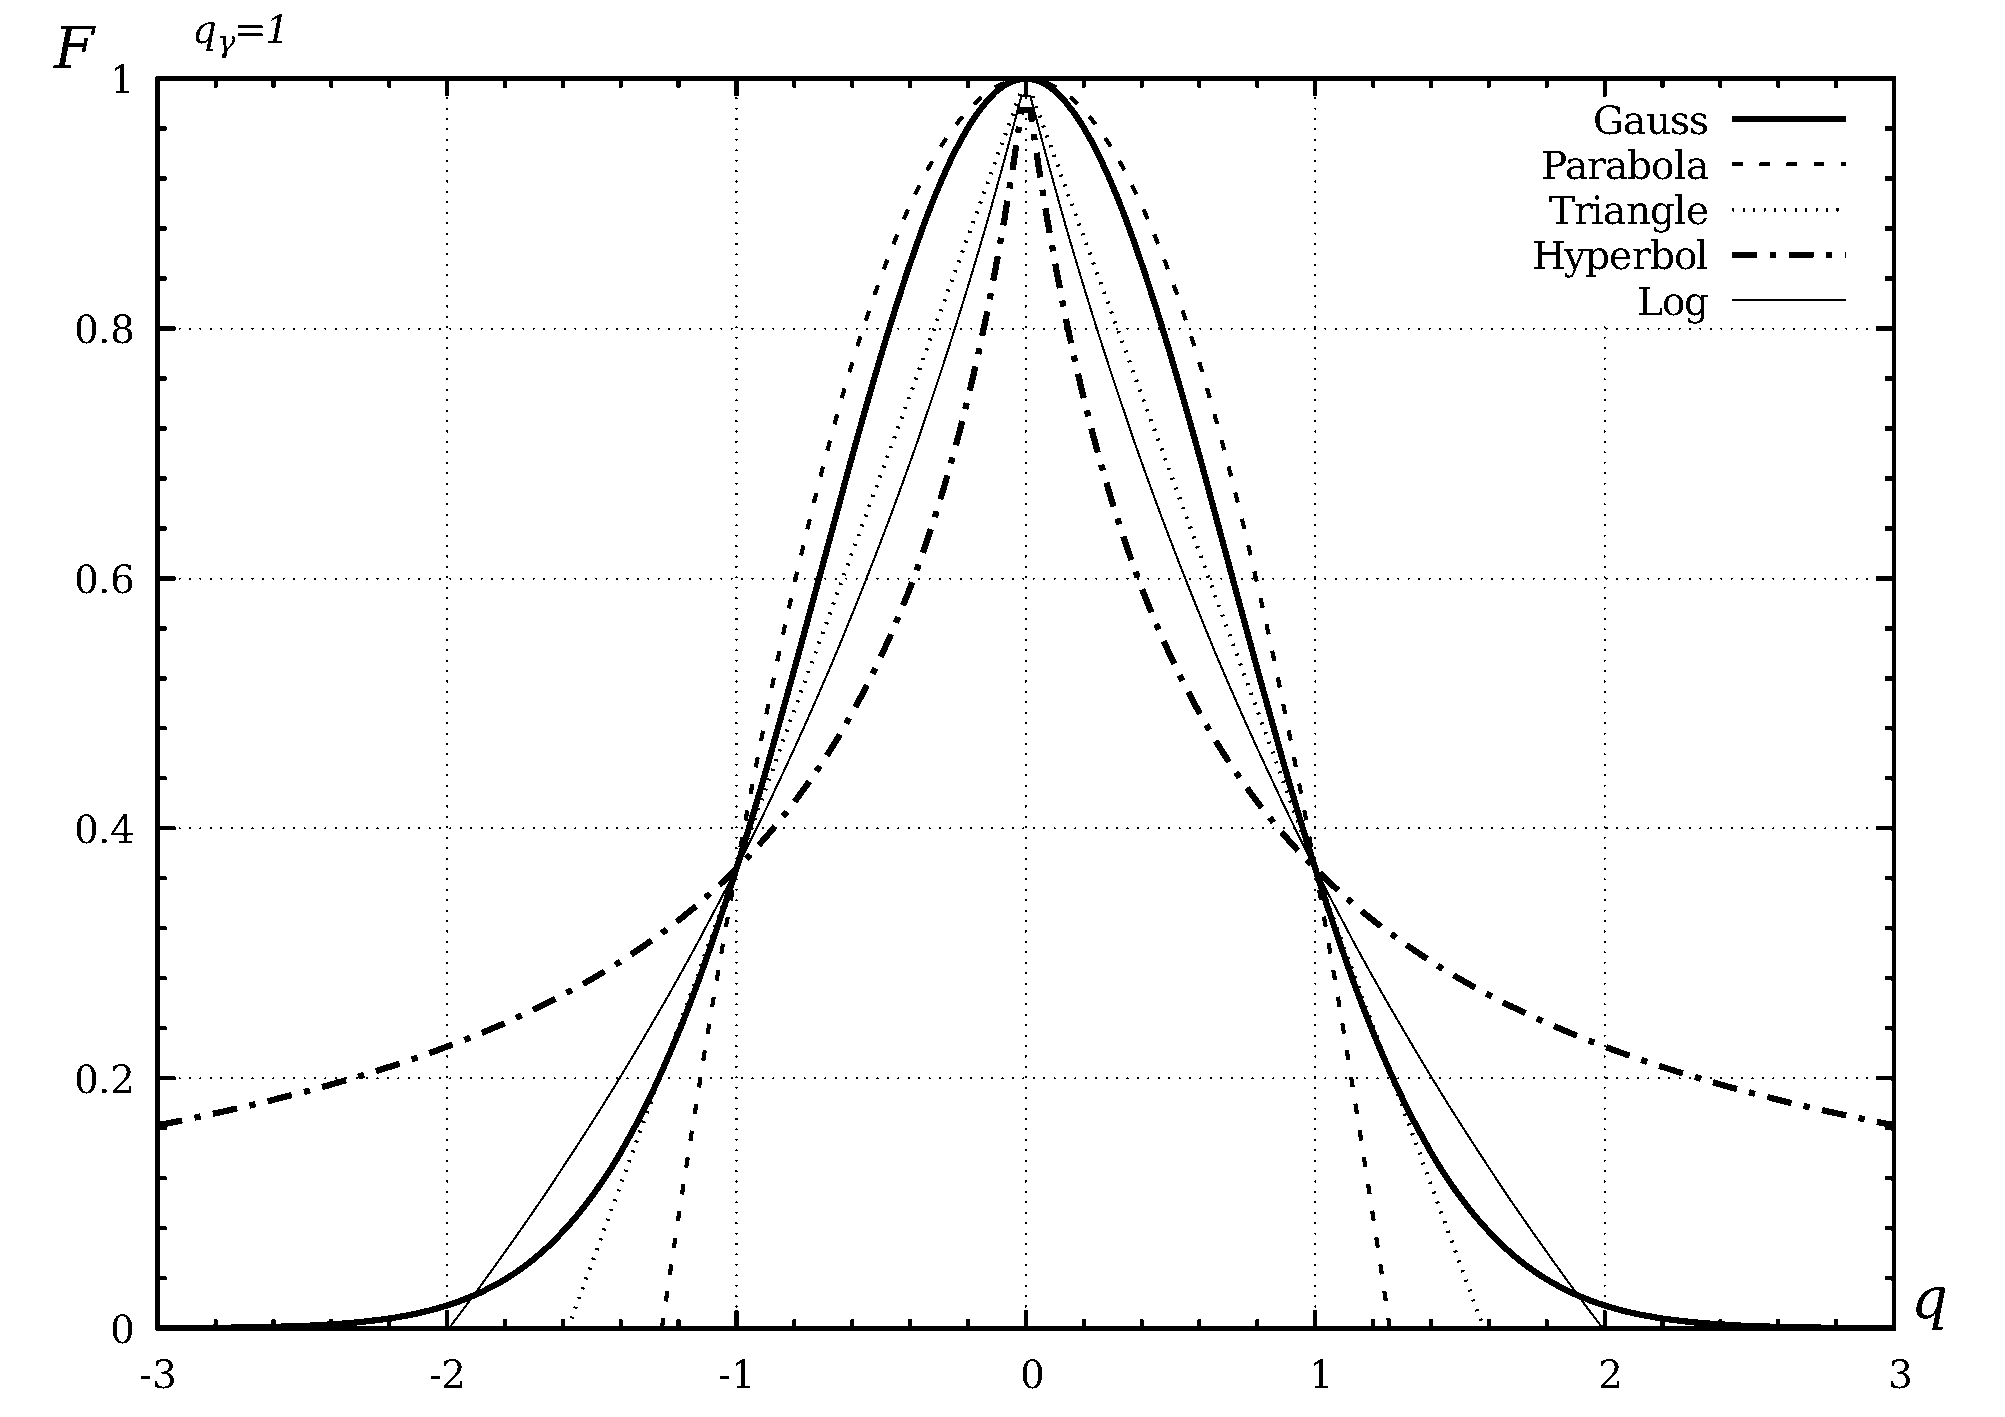
\includegraphics[width=55\TW]{../p3/p/F_types.png}
    \caption{Функції якості ідентифікації (\ref{atu:eq:F_gauss})--(\ref{atu:eq:F_log})}
    \label{atu:f:F_types}
  \end{figure}
  \end{tabular}

 $q_\gamma$\label{atu:d:q_gamma}
  --- величина, обернена до чутливості функції якості $\gamma$,
  задає масштаб і робочий діапазон функції якості.


\end{frame}


% -----------------------------------------------------------------------

\begin{frame}
  \frametitle{~}
  %\framesubtitle{}

  \Xhead{Структура пошукових систем}

  Визначення:
  \textbf{пошуковий агент} --- це динамічна система, яка отримує вихідні ($x(t)$),
  і, при необхідності, вхідні ($u(t)$) сигнали від однієї або кількох моделей,
  величину оцінки стану об'єкта за критерієм ідентифікації,
  може обмінюватися інформацією з іншими елементами пошукової системи,
  та, на підставі значення критерію
  ідентифікації, реалізує алгоритм настройки параметрів моделі (моделей) таким
  чином, щоб забезпечити визначення заданого параметра.

  \medskip

  Визначення:
  \textbf{координатор пошуку} --- це динамічна система, яка отримує інформацію
  від пошукових агентів і на підставі цієї інформації визначає
  $p_{\mathrm{id}}(t)$ --- величину ідентифікованого параметра.
  Крім цього, координатор може, на підставі цієї ж інформації,
  керувати процесом адаптації всієї пошукової системи.


  \begin{figure}[htb!]
    \begin{center}
      % vi:syntax=tex
\begin{tikzpicture}
  %\draw[hair,step=1.0em] (0,-3) grid (12.0,3.0);
  \bXStyleBloc{semiboldline,inner sep=2pt};
  \bXLineStyle{medline};
  % --- U
  \bXInput{U};
  \path (U.center) ++(0.9em,0.0em) coordinate (UxM);
  \fill (UxM) circle[radius=0.05];
  %\bXLinkName[0.5]{U}{$u(t)$};
  % --- M1
  \bXBlocL[3.0]{M1}{$\mathbf{M}_1$}{U};
  \bXLink[$u(t)$]{U}{M1}; %% node 'U-M1' is here
  \path (M1.east) ++(0.0,-1.0em) coordinate (Mxm1);
  % --- A1
  \bXBloc[10.0]{A1}{$A_{1}$}{M1};
  \path (A1.west) ++(0.0,-1.0em) coordinate (Axm1);
  \path (A1.west) ++(0.0,+1.0em) coordinate (Aqo1);
  \path (Aqo1) ++(-1.0em,0.0em) coordinate (Aqoi1) {};  % external input
  \draw[medlinep] (Aqoi1) -- (Aqo1);
  \fill (Aqoi1) circle[radius=0.05];
  \bXLink[$x_{1}(t)$]{Mxm1}{Axm1};
  \draw[infoline,<->] (A1.40) -- ++(3.0em,0.0em);
  \draw[medlinep] (A1.east) -- ++(3.0em,0.0em);
  \node[above right] at(A1.east) {$p_1(t)$};
  \draw[medlinep] (A1.east) -- ++(0.5em,0.0em) -- ++(0.0em,-2.0em) -| (M1.south);
  \draw[infoline,->] (A1.south) -- ++(0.0em,-0.8em);
  \path (A1.east)  ++(6.0em,-1.0em) coordinate (Pout);
  \draw[medlinep] (Pout) -- ++(2.0em,0.0em);
  \node[above right] at (Pout) {$p_{\mathrm{id}}(t)$};
  % --- M0
  \bXBranchy[-4]{UxM}{U0};
  \bXBloc[2.1]{M0}{$\mathbf{M}_0$}{U0};
  \path (M0.east) ++(0.0,-1.0em) coordinate (Mxm0);
  \bXLinkyx{UxM}{M0};
  % --- A0
  \bXBloc[10.0]{A0}{$A_{0}$}{M0};
  \path (A0.west) ++(0.0,-1.0em) coordinate (Axm0);
  \path (A0.west) ++(0.0,+1.0em) coordinate (Aqo0);
  \path (Aqo0) ++(-1.0em,0.0em)  coordinate (Aqoi0) {};  % external input
  \fill (Aqoi0) circle[radius=0.05];
  \draw[medlinep] (Aqoi0) -- (Aqo0);
  \bXLink[$x_{0}(t)$]{Mxm0}{Axm0};
  \path (A0.north east)        ++(3.0em,0.0em) coordinate (AAlt);
  \draw[infoline,<->] (A0.40) -- ++(3.0em,0.0em);
  \draw[medlinep] (A0.east) -- ++(3.0em,0.0em);
  \node[above right] at(A0.east) {$p_0(t)$};
  \draw[medlinep] (A0.east) -- ++(0.5em,0.0em) -- ++(0.0em,-2.0em) -| (M0.south);
  \draw[infoline,<->] (A0.south) -- (A1.north);
  % --- Obj
  \bXBranchy[-8]{UxM}{UO};
  \bXBloc[2.1]{Obj}{$\mathbf{O}$}{UO};
  \bXLinkyx{UxM}{Obj};
  \bXCompSum[3.0]{W}{Obj}{}{}{}{};
  \bXLink{Obj}{W};
  \draw[medline,<-] (W.north) -- ++(0.0em,1.0em) node[right] {$w(t)$};
  \bXBloc[2.5]{Qo}{$q$}{W};
  \bXLink[$x_o(t)$]{W}{Qo};
  \node[above right] at (Qo.east) {$q_o(t)$};
  %
  % --- Mn
  \bXBranchy[6]{UxM}{Un};
  \bXBloc[2.1]{Mn}{$\mathbf{M}_{n-1}$}{Un};
  \path (Mn.east) ++(0.0,-1.0em) coordinate (Mxmn);
  \bXLinkyx{UxM}{Mn};
  \draw[dotted,boldline] (M1.south) ++(0.0em,-1.0em) -- (Mn.north);
  % --- An
  \bXBloc[10.0]{An}{$A_{n-1}$}{Mn};
  \path (An.west) ++(0.0,-1.0em) coordinate (Axmn);
  \path (An.west) ++(0.0,+1.0em) coordinate (Aqon);
  \path (Aqon) ++(-1.0em,+0.0em) coordinate (Aqoin) {};  % external input
  \draw[medlinep] (Aqoin) -- (Aqon);
  \draw[medline] (Qo) -| (Aqoin);
  \bXLink[$x_{n-1}(t)$]{Mxmn}{Axmn};
  \path (An.south east) ++(6.0em,0.0em) coordinate (AArb);
  \draw[infoline,<->] (An.40) -- ++(3.0em,0.0em);
  \draw[medlinep] (An.east) -- ++(3.0em,0.0em);
  \node[above right] at(An.east) {$p_{n-1}$};
  \draw[medlinep] (An.east) -- ++(0.5em,0.0em) -- ++(0.0em,-2.0em) -| (Mn.south);
  \draw[infoline,->] (An.north) -- ++(0.0em,0.5em);
  %
  \draw[semiboldline] (AAlt) rectangle (AArb);
  %
  \draw[white,dotted,line width=3.0pt] (UxM) ++(0.0em,-1.0em) -- ++(0.0em,-4.0em);
  %
  \bXStyleBlocDefault;
  \bXDefaultLineStyle;
  %
  \TikzAddPadding
  %
\end{tikzpicture}

    \end{center}
    \caption{Мультиагентна система ідентифікації з плоскою структурою}
    \label{atu:f:agents_flat}
  \end{figure}

  Таким чином, система ідентифікації складається з множини агентів, та
  множини координаторів пошуку, які спільно вирішують задачу ідентифікації.
  За винятком ієрархічних систем ідентифікації, найчастіше використовується один координатор пошуку.

\end{frame}

% -----------------------------------------------------------------------

\begin{frame}
  \frametitle{~}
  %\framesubtitle{}

  \Xhead{Конфігурації агентів і координаторів}

\textbf{Рій} --- множина агентів, що забезпечує ідентифікацію за рахунок
концентрації максимальної кількості агентів в області передбачуваного максимуму
функції якості або ж заданого значення критерію. Три складові поведінки: рух
до оцінюваного локального екстремуму, до глобального, випадкова складова.

\textbf{Стрій} --- множина агентів, розташування яких, і якщо необхідно,
зміщення, задається однаковим чином. Відсутня індивідуальна динаміка кожного
агента. Нерухомий стрій утворює \textbf{сітку},
як рівномірно розподілену по простору параметрів, так і~ні.

\textbf {Ансамбль} ---
множина агентів, що забезпечує ідентифікацію за рахунок розподілу агентів таким
чином, який забезпечує як точність ідентифікації за рахунок обмеженого
скупчення агентів в областях передбачуваних максимумів функції якості, так і оперативного
переключення на інші області при зміні параметрів за рахунок недопущення
невиправданої скупченості агентів.

  \begin{figure}[htb!]
    \begin{center}
      % vi:syntax=tex
\begin{tikzpicture}
  \bXStyleBloc{semiboldline,inner sep=2pt};
  \bXLineStyle{medline};
  % --- U
  \bXInput{U};
  % --- M
  \bXBlocL[2.0]{M}{$\mathbf{M}_i$}{U};
  \bXLink[$u(t)$]{U}{M};
  % --- Q
  \bXBloc[3.5]{Q}{$q$}{M};
  \path (Q.east) ++(0.0,-1.0em) coordinate (Qqm);
  \path (Q.south west) ++(-0.3,-0.4) coordinate (BLKlb);
  \bXLink[$x_i(t)$]{M}{Q};
  % --- F
  \bXBloc[2.5]{F}{$F(q_o,q_{mi})$}{Q};
  \path (F.west) ++(0.0,-1.0em) coordinate (Fqm);
  \path (F.west) ++(0.0,+1.0em) coordinate (Fqo);
  \path (Fqo) ++(-1.6em,+2.8em) coordinate (Fqoi) {};  % external input
  \draw[medlinep] (Fqoi) |- (Fqo);
  \node[below right] at (Fqoi) {$q_o(t) \qquad A_i$};
  \bXLink[$q_i(t)$]{Qqm}{Fqm};
  % --- P
  \bXBloc[2]{P}{$P$}{F};
  \draw[infoline,<->] (P.north) -- +(0,0.8);
  \path (P.north east) ++(0.1,+0.4) node (BLKrt) {};
  \bXLink[$F_i(t)$]{F}{P};
  % -- output
  \bXOutput[2.8]{Po}{P};
  \bXLink[$p_i(t)$]{P}{Po};
  \bXOutput[1.0]{Por}{P};
  \fill(Por) circle[radius=0.05];
  \bXLineStyle{semiboldline};
  \bXReturn{Por}{M}{$p_i(t)$};
  % -- block
  \draw[subelem] (BLKlb) |- (BLKrt) |- (BLKlb);
  \bXStyleBlocDefault;
  \bXDefaultLineStyle;
  %
  \TikzAddPadding
  %
\end{tikzpicture}

    \end{center}
    \caption{Пошуковий агент, який використовую функцію якості $F$, та управляє параметром однієї моделі}
    \label{atu:f:agent1}
  \end{figure}


  \begin{figure}[htb!]
    \begin{center}
      % vi:syntax=tex
\begin{tikzpicture}
  \bXStyleBloc{semiboldline,inner sep=2pt};
  \bXLineStyle{medline};
  % --- U
  \bXInput{U};
  % --- M
  \bXBlocL[2.0]{M}{$\mathbf{M}_i$}{U};
  \bXLink[$u(t)$]{U}{M};
  % --- Q
  \bXBloc[3.5]{Q}{$q$}{M};
  \path (Q.east) ++(0.0,-1.0em) coordinate (Qqm);
  \path (Q.south west) ++(-0.3,-0.4) coordinate (BLKlb);
  \bXLink[$x_i(t)$]{M}{Q};
  % --- P
  \bXBloc[2]{P}{$P$}{Q};
  \draw[infoline,<->] (P.north) -- +(0,0.8);
  \path (P.west) ++(0.0,-1.0em) coordinate (Pqm);
  \path (P.west) ++(0.0,+1.0em) coordinate (Pqo);
  \path (Pqo) ++(-1.6em,+2.8em) coordinate (Pqoi) {};  % external input
  \path (P.north east) ++(0.1,+0.4) node (BLKrt) {};
  \bXLink[$q_{i}(t)$]{Qqm}{Pqm};
  \draw[medlinep] (Pqoi) |- (Pqo);
  \node[below right] at (Pqoi) {$q_o(t) \qquad A_i$};
  %\bXLink[$F_i(t)$]{F}{P};
  % -- output
  \bXOutput[2.8]{Po}{P};
  \bXLink[$p_i(t)$]{P}{Po};
  \bXOutput[1.0]{Por}{P};
  \fill(Por) circle[radius=0.05];
  \bXLineStyle{semiboldline};
  \bXReturn{Por}{M}{$p_i(t)$};
  % -- block
  \draw[subelem] (BLKlb) |- (BLKrt) |- (BLKlb);
  \bXStyleBlocDefault;
  \bXDefaultLineStyle;
  %
  \TikzAddPadding
  %
\end{tikzpicture}

    \end{center}
    \caption{Пошуковий агент, який використовую критерій $q$, та управляє параметром однієї моделі}
    \label{atu:f:agent1q}
  \end{figure}

\end{frame}


% -----------------------------------------------------------------------

\begin{frame}
  \frametitle{~}
  %\framesubtitle{}

  \Xhead{}

  Вихідними сигналами агента є:

  \begin{itemize}

    \item
      $p_c(t)$ ---
      поточне значення параметра.

    \item
      $p_e(t)$\label{atu:d:p_e} --
      поточне значення оцінки параметра.

    \item
      $F_c(t)$ ---
      поточне значення функції якості (якщо використовується одна
      модель для агента, або ж якщо агент якимось чином її усереднює
      або апроксимує в разі декількох моделей). Може поєднувати
      функції вхідного і вихідного сигналів.

    \item
      $q_c(t)$ ---
      значення критерію якості (аналогічно попередньої величиною в
      разі декількох моделей); спочатку цей сигнал був представлений
      як вхідний для агента, проте він може використовуватися і
      на більш високих рівнях системи ідентифікації. Якщо ж агенту
      значення критерію недоступно, то і в списку вихідних сигналів
      ця величина також відсутня.

    \item
      $F_e(t)$ ---
      апроксимоване значення функції якості в точці
      $p_e(t)$. Якщо агент не використовує для роботи апроксимацію
      $F$, то і відповідний вихідний сигнал не використовується.

    \item
      $S(t)$ ---
      ступінь ``впевненості'' агента в отриманому значенні.

    \item
   $W(t) = F_c(t) S(t)$ --- worthiness.
  \end{itemize}

%
\begin{equation}
  S_1 = c_\mathrm{su} \exp \left( - \frac{ \big( k_l c_\mathrm{dist} ( p_e - p_c ) \big)^2 }{p_b^2} \right)
  ,
  \label{atu:eq:S1}
\end{equation}
%
\begin{equation}
  S_3 = c_\mathrm{su} \exp \left( - \frac{ \big( k_l c_\mathrm{dist} \min( |p_e - p_l|,|p_e - p_c|, |p_e - p_r| ) \big)^2 }{p_b^2} \right)
  .
  \label{atu:eq:S3}
\end{equation}
%
де
$c_\mathrm{su}$ ---
коефіцієнт, що відображає працездатність методу в даному випадку;
$c_\mathrm{dist}$ ---
коефіцієнт, що визначає ``штраф'' або ``бонус'', пов'язаний з відносним розташуванням робочих точок;
$k_l$ ---
коефіцієнт оцінки нелінійності системи;
$p_b$
--- характерний масштаб, щодо якого враховується видалення $p_e$ від використаних точок.

\end{frame}


% -----------------------------------------------------------------------

\begin{frame}
  \frametitle{~}
  %\framesubtitle{}

  \Xhead{Методи агентів, які використовують значення критерію}

  1 модель: використовуємо історію. \\
  2 моделі: можемо оцінити $p_e$ за лінійним наближенням. \\
  3 моделі: можемо оцінити $p_e$ + ``впевненість'' $S_e$.

  Якщо
  $F_c > F_\mathrm{good}$, то $p_e = p_c$, $S=1$.

  Якщо
  $F_c \le F_\mathrm{good}$, то $q_o -q_c \ne 0$,
  і можна застосувати наступні перетворення:
  %
  \[
    \tilde{p}_l = p_l - p_c;
  \quad
  \tilde{p}_c = p_c - p_c = 0;
  \quad
  \tilde{p}_r = p_r - p_c;
  \quad
  \tilde{p}_e = p_e - p_c;
\]
  \begin{equation}
    \tilde{q}_l = \frac{q_l-q_c}{q_c-q_o};
    \quad
    \tilde{q}_c = \frac{q_c-q_o}{q_c-q_o} = 1;
    \quad
    \tilde{q}_l = \frac{q_l-q_c}{q_c-q_o}.
    \label{atu:eq:q_agent_rel}
  \end{equation}

  \begin{equation}
    \tilde{p}_{el} = \frac{\tilde{p}_l}{1-\tilde{q}_l},
    \quad
    \tilde{p}_{er} = \frac{\tilde{p}_r}{1-\tilde{q}_r}.
    \label{atu:eq:pr_ex}
  \end{equation}

  Найкращий випадок,  дві послідовні точки
  розташовані по один бік
  від прямої
  $q = q_o$, а решта --- по інший.

  \begin{figure}[htb!]
    \centerline{
      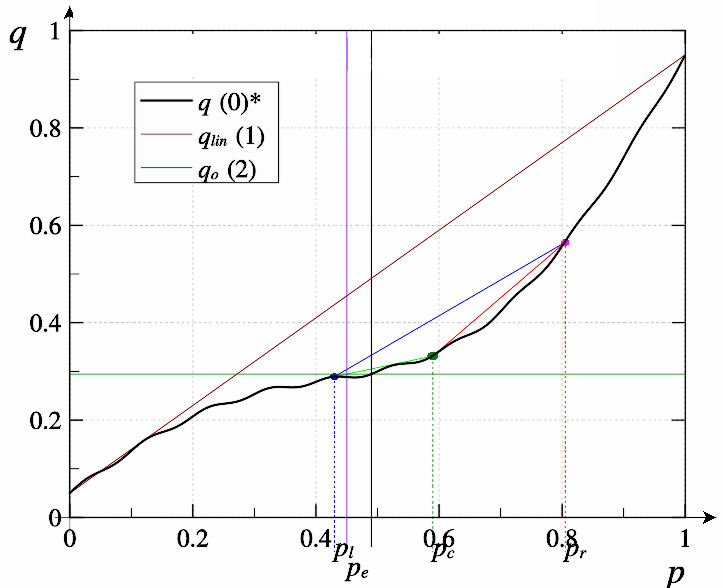
\includegraphics[width=49\TW]{../p3/p/pq_sin-p_pq_po=049_xl.png}
    \hfill
    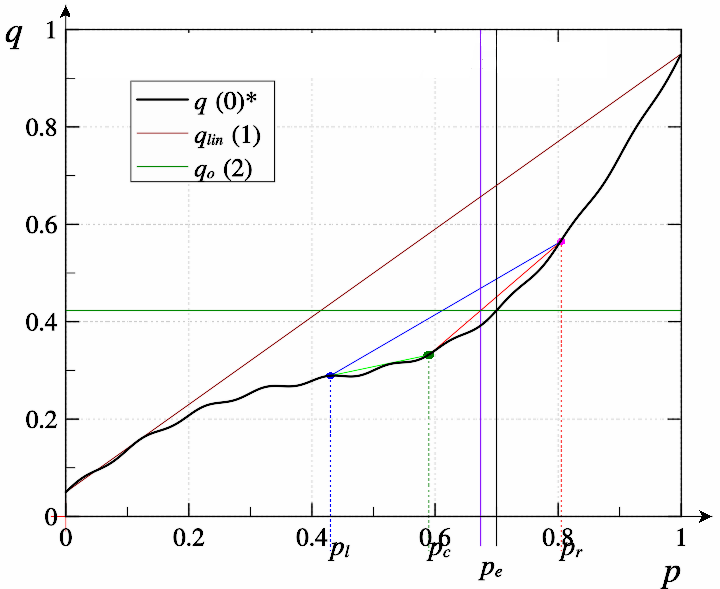
\includegraphics[width=49\TW]{../p3/p/pq_sin-p_pq_po=070_xl.png}
    }
    \caption{Визначення точки $p_e$ методом $p_{eql}$ при $p_o \in [p_l, p_r]$}
    \label{atu:f:pq_4}
  \end{figure}

  % У цьому найсприятливішому випадку проводиться інтерполяція, а не екстраполяція
  % залежності $q(p)$, і досить вибрати ту ділянку, на якій гарантовано
  % відбувається перетин. При цьому значення всіх коефіцієнтів підкреслюють
  % впевненість агента в значенні $p_e$, що отримано:

  \vspace{-7ex}

  \begin{equation}
    \tilde{p}_e
    =
    \begin{cases}
      \tilde{p}_{el}, & \tilde{q}_l < 0
      \\
      \tilde{p}_{er}, & \text{ otherwise}.
    \end{cases}
    ,
    c_\mathrm{su} = 1.0, \;  c_\mathrm{dist} = 0.5,  \;
    p_b =
    \begin{cases}
      -\tilde{p}_l, & \tilde{q}_l < 0
      \\
      \tilde{p}_r, & \text{ otherwise}.
    \end{cases}.
    \label{atu:eq:pr_e4}
  \end{equation}

  Останні випадки,
  характеризуються меншою ``упевненістю'' в отриманому значенні $p_e$,
  що відображається у коефіцієнтах
  $c_\mathrm{su}$, $c_\mathrm{dist}$ та  $p_b$.

  Цій метод означимо як $p_{eql}$.

\end{frame}



% -----------------------------------------------------------------------

\begin{frame}
  \frametitle{~}
  %\framesubtitle{}

  \Xhead{Методи для агентів, які використовують значення функції якості}

  Три сусідніх агента, які взаємодіють між собою, здатні не тільки оцінити градієнт
  функції якості у власному околі, а й визначити наявність там
  максимуму.
  %
  \[
    \tilde{p}_c = 0, \,
    \tilde{p}_l = p_l - p_c, \,
    \tilde{p}_r = p_r - p_c.
  \]
  %
  \[
    \tilde{F}_c = 0, \,
    \tilde{F}_l = F_l - F_c, \,
    \tilde{F}_r = F_r - F_c.
  \]
    %
    \[
    \left\{
      \begin{array}{l}
        a_2 \tilde{p}_l^2 + a_1 \tilde{p}_l  = \tilde{F}_l
        \\
        a_2 \tilde{p}_r^2 + a_1 \tilde{p}_r  = \tilde{F}_r
      \end{array}
    \right. .
  \]

  \begin{equation}
    a_1 = \frac{\tilde{F}_r \tilde{p}_l^2 - \tilde{F}_l \tilde{p}_r^2 }
              { \tilde{p}_l^2 \tilde{p}_r  - \tilde{p}_l \tilde{p}_r^2 },
    \;
    a_2 = - \frac{\tilde{F}_r \tilde{p}_l - \tilde{F}_l \tilde{p}_r }
               { \tilde{p}_l^2 \tilde{p}_r  - \tilde{p}_l \tilde{p}_r^2 },
    \;
    \tilde{p}_e = - \frac{a_1}{2 a_2};
    \;
    p_e = p_c - \frac{a_1}{2 a_2}.
    \label{atu:eq:p_eFq}
  \end{equation}

  При $a_2<0$, $p_o \in [p_l,p_r]$:

  \begin{figure}
    \PicDoubleNL{../p3/p/p_eFq/q_p_eFq_p49_xl.png}{../p3/p/p_eFq/q_p_eFq_p70_xl.png}
    \caption{Визначення точки $p_e$ методом $p_{eFq}$ при $p_o \in [p_l, p_r]$}
    \label{atu:f:p_eFq_intra}
  \end{figure}

  Визначення $p_e$ по (\ref{atu:eq:p_eFq}) будемо позначати як $p_{eFq}$.

  Оцінювання $p_e$ методом COG за значеннями функції якості:
 %
 \begin{equation}
   p_e =
   \frac{p_l F_l + p_c F_c + p_r F_r}{ F_r + F_c + F_r}  .
   \label{atu:eq:p_eFc}
 \end{equation}

Умова обмеженості оцінки $p_e \in [p_l; p_r]$ в цьому випадку виконується
автоматично. Визначення $p_e$ по (\ref{atu:eq:p_eFc}) в подальшому будемо позначати $p_{eFc}$.

\end{frame}


% -----------------------------------------------------------------------

\begin{frame}
  \frametitle{~}
  %\framesubtitle{}

  % \Xhead{}
  Демонстраційна штучна залежність~$q(p)$:
  %
  \begin{equation}
    q_\mathrm{dem}(p) = q_{00} + c_\mathrm{lin} \tilde{p} + c_\mathrm{s1} \sin( \pi \tilde{p} ) + c_\mathrm{s2} \sin( 2 \pi \tilde{p} ) + c_\mathrm{s20} \sin( 20 \pi \tilde{p} ),
    \label{atu:eq:q_dem}
  \end{equation}
  %
  де $q_{00}$, $c_\mathrm{lin}$, $c_\mathrm{s1}$, $c_\mathrm{s2}$, $c_\mathrm{s20}$
  ---
  коефіцієнти, що дозволяють налаштувати цю залежність для перевірки заданого аспекту поведінки агента,
  $\tilde{p} = \frac{p - p_{\min}}{p_{\max} - p_{\min}}$.

  \begin{figure}
    \PicTriple{../p3/p/qls_pe-p_po_qg_eql_all_xl.png}{../p3/p/qls_pe-p_po_qg_eFq_all_xl.png}{../p3/p/qls_pe-p_po_qg_eFc_all_xl.png}
    \caption{Залежності $e(p_o,q_\gamma)$ для методів $p_{eql}$ (a), $p_{eFq}$ (b), $p_{qFc}$ (c) при повному комплекті нелінійних членів}
    \label{atu:f:qsl_pe_po_qg_all}
  \end{figure}

  \begin{figure}
    \PicTriple{../p3/p/qls_pe-p_po_qg_Sql_all_xl.png}{../p3/p/qls_pe-p_po_qg_SFq_all_xl.png}{../p3/p/qls_pe-p_po_qg_SFc_all_xl.png}
    \caption{Залежності $S(p_o,q_\gamma)$ для методів $p_{eql}$ (a), $p_{eFq}$ (b), $p_{qFc}$(c)}
    \label{atu:f:qsl_S_po_qg_all}
  \end{figure}

  \vspace{-3ex}

  \begin{figure}[htb!]
    \PicTriple{../p3/p/qls_pe-p_A_qg_eql_all_xl.png}{../p3/p/qls_pe-p_A_qg_eFq_all_xl.png}{../p3/p/qls_pe-p_A_qg_eFc_all_xl.png}
    \caption{Залежності $e(A,q_\gamma)$ для методов $p_{eql}$ (a), $p_{eFq}$ (b), $p_{qFc}$ (c)}
    \label{atu:f:qsl_pe_A_qg_all}
  \end{figure}
\end{frame}


% -----------------------------------------------------------------------

\begin{frame}
  \frametitle{~}
  %\framesubtitle{}

  \Xhead{Динаміка пошукових агентів}

  Визначення ``сил'': \\
  $f_e$ ---
  ``сила тяжіння'' до локальної оцінки $p_e$:
  \begin{equation}
    f_e(t) = - k_e \left( p_c(t) - p_e(t) \right)  ,
    \label{atu:eq:f_e_lin}
  \end{equation}
  \begin{equation}
    f_e(t) = - k_e W(t) \left( p_c(t) - p_e(t) \right) ,
    \label{atu:eq:f_e_lin_W}
  \end{equation}

  ``Сила'' $f_n$ визначає взаємодію агента з найближчими сусідами.
  %
  \begin{equation}
    f_n = k_n ( p_r - 2 p_c + p_l ),
    \label{atu:eq:f_n_lin}
  \end{equation}
  \begin{equation}
    f_n = k_n \left( \log\left( \frac{p_r-p_c}{p_{d0}} \right) -  \log\left( \frac{p_c-p_l}{p_{d0}}\right) \right),
    \label{atu:eq:f_n_log}
  \end{equation}
  %
  де
  $p_{d0}$ ---
  базова відстань між агентами.

 ``$f_c$'' --- ``сила тяжіння'' до початкового значення параметра ($p_{c}(0)$)
 %
  \begin{equation}
    f_c = -k_c (p_c - p_{c}(0)) ,
    \label{atu:eq:f_c}
  \end{equation}
  %
  \begin{equation}
  f_t = f_c + f_n + f_e .
  \label{atu:eq:f_t}
\end{equation}

  Можна використовувати різні способи визначення пошукової динаміки агента при
  заданій силі. Наприклад, метод ``важкої кульки'':
  \begin{equation}
    m \ddot{p}_c + \nu \dot{p}_c = f_t(t),
    \label{atu:eq:heavy_ball}
  \end{equation}
  %
  де $m$ --- еквівалент маси кульки, $\nu$ --- коефіцієнт умовної в'язкості.

  Також може використовуватися наближення динаміки тіла у в'язкій рідині, коли
  вплив інерції дуже малий в порівнянні з в'язкістю, при цьому зміни параметрів
  моделей (пошукових агентів) задаються наступним чином:
  %
  \begin{equation}
    \od{p_c}{t} = v_f f_t(t),
    \label{atu:eq:v_f}
  \end{equation}
  %
  де $f_t$ --- сума всіх діючих ``сил'',
  $v_f = 1 / \nu$ --- коефіцієнт
  пропорційності.
\end{frame}


% -----------------------------------------------------------------------

\begin{frame}
  \frametitle{~}
  %\framesubtitle{}

  \Xhead{Методи визначення пошуковим координатором значення ідентифікованого параметра}

``Best:''
\begin{equation}
  p_{bcF}
  =
  p_{c,i};
  \quad
  i : F_i = \max{F_j}, \quad j=0 \ldots N-1 .
  \label{atu:eq:p_bcF}
\end{equation}
%
Аналогічно визначаються залежності
$p_{bcS}$ та $p_{bcW}$. Якщо замість $p_c$ використовувати $p_e$ ---
$p_{bcF}$ $p_{bcS}$ та $p_{bcW}$.

\vfill

``Global COG:''
%
\begin{equation}
  p_{gcF}
  =
  \frac{\sum\limits_{i=0}^{N-1} F_{i} p_{i}}
       {\sum\limits_{i=0}^{N-1} F_{i} }
  .
  \label{atu:eq:p_gcF}
\end{equation}
%
Аналогічно визначаються методи
$p_{gcS}$,
$p_{gcW}$,
$p_{geF}$,
$p_{geS}$ та
$p_{geW}$.

\vfill

``Local COG:''
%
\begin{equation}
  p_{leF}
  =
  \frac{ F_{l} p_{l} + F_{c} p_{c} + F_{r} p_{r} }
       { F_{l}       + F_{c}       + F_{r}       }
  .
  \label{atu:eq:p_lcFl}
\end{equation}
%
Аналогічно визначаються методи
$p_{lcS}$,
$p_{lcW}$,
$p_{leF}$,
$p_{leS}$ та
$p_{leW}$.

\Xhead{Похибки та якість ідентифікації:}

\begin{equation}
  e_{gcF}(t) = p_{gcF}(t) - p_o(t),
  \quad
  \ldots
  \quad
  e_{leW}(t) = p_{leW}(t) - p_o(t).
  \label{atu:eq:e_xx}
\end{equation}

\begin{equation}
  \overline{e} = \mu( p_o(t), p_\mathrm{id}(t) ),
  \quad
  t \in [0;T].
\label{atu:eq:e_mu}
\end{equation}

\begin{equation}
  \overline{e}_{00}
  =
  \overline{e}\left(p_o(t),p_{00}\right),
  \quad
  p_{00} \text{ --- центр  множини } \mathcal{P}.
  \label{atu:eq:e_00}
\end{equation}

\begin{equation}
  \overline{e}_{rbcF} = \frac{\overline{e}_{bcF}}{\overline{e}_{00}}, \;
  \overline{e}_{rleS} = \frac{\overline{e}_{leS}}{\overline{e}_{00}}, \;
  \overline{e}_{rgeW} = \frac{\overline{e}_{geW}}{\overline{e}_{00}},
  \quad \ldots \quad
  \overline{e}_{rqeF} = \frac{\overline{e}_{qeF}}{\overline{e}_{00}}.
  \label{atu:eq:e_rxx}
\end{equation}

\begin{equation}
  \overline{e}_{rblcS} = \frac{\overline{e}_{lcS}}{\overline{e}_{bc}},
  \quad \ldots \quad
  \overline{e}_{rbqeW} = \frac{\overline{e}_{qeW}}{\overline{e}_{bc}} \text{ on }  (v_f=0) .
  \label{atu:eq:e_rbxx}
\end{equation}


\end{frame}


% -----------------------------------------------------------------------

\begin{frame}
  \frametitle{~}
  %\framesubtitle{}

  \Xhead{Класифікація систем пошукової ідентифікації}

  \begin{enumerate}

    \item
      Перший символ (``F'', ``q'', ``x'' ) визначає,
      яка величина використовується кожним агентом для визначення $p_e$.

    \item
      Другий символ (``l'' --- linear, ``q'' --- quadratic \ldots ) 
      задає спосіб визначення величини $p_e$ одним агентом.

    \item
      Третій символ визначає локальну пошукову геометрію, найчастіше --- кількість
      агентів в в пошуковій групі, наприклад: ``2'' --- пошукова пара, ``3'' --- триплет.

    \item
      Четвертий символ (``z'' --- zero, ``r'' --- real \ldots),
      описує поведінку додаткових моделей, які розташовані на границі:

    \item
      П'ятий символ (``c'' --- const, ``l'' --- linear \ldots )
      позначає обрану залежність для величини $f_e$ (або
      аналогічної величини, якщо $f_e$ безпосередньо не використовується).

    \item
      Шостий символ (``o'' --- one, ``F'', ``S'', ``W'') визначає множник,
      що використовується для величини $f_e$ при визначенні динаміки об'єкта.

    \item
      Сьомий символ (``z'' --- zero, ``v'' --- viscous \ldots)
      вказує, яким чином величина $f_t$ (або її еквівалент) впливає на динаміку агента.

    \item
      Восьмий (``n'' --- none, ``t'' --- triangle \ldots ) символ дозволяє вказати,
      який додатковий пошуковий рух реалізує агент.

    \item
      Дев'ятий символ задає спосіб визначення ідентифікованого параметра по всьому ансамблю (``b'', ``g'', ``l'', ``q'').


    \item
      Десятий символ (``c'', ``e'') визначає, який з вихідних сигналів пошукового агента використовується.

    \item
      Одинадцятий символ (``F'', ``S'', ``W'') вказує,
      яка величина використовується для визначення ваги кожного агента.


  \end{enumerate}

Приклад позначень:
``Fc3zlovngcW.$q_{x^2}$'',
``ql3ruWvnAeF'',
``xl2nlosdlcA''.

\end{frame}


% -----------------------------------------------------------------------

\begin{frame}
  \frametitle{~}
  %\framesubtitle{}

  \Xhead{Тестові умови: залежність  (\ref{atu:eq:q_dem}) та}

  \begin{equation}
    p_o(t) = p_0 +  U_{p} \sign \sin( \omega_{p} t ),
    \label{atu:eq:po_t_sign}
  \end{equation}

  \begin{equation}
    p_o(t) = p_0 +  U_{p} \sin( \omega_{p} t ).
    \label{atu:eq:po_t_sin}
  \end{equation}

  \begin{equation}
    p_o(t) = p_0 +  U_{p} \frac{t}{T}.
    \label{atu:eq:po_t_ramp}
  \end{equation}

  \Xhead{Рівноважні конфігурації пошукових агентів}

  \begin{figure}[htb!]
    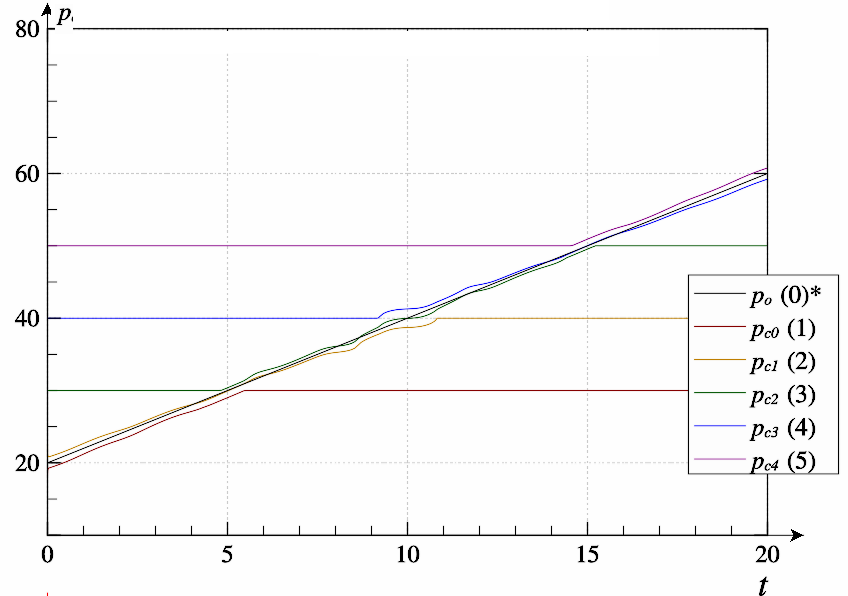
\includegraphics[width=\DDP]{../p3/p/ramp/qls-p_t_pi_Fq3rlovnAAF_ramp_xl.png} \hfill
    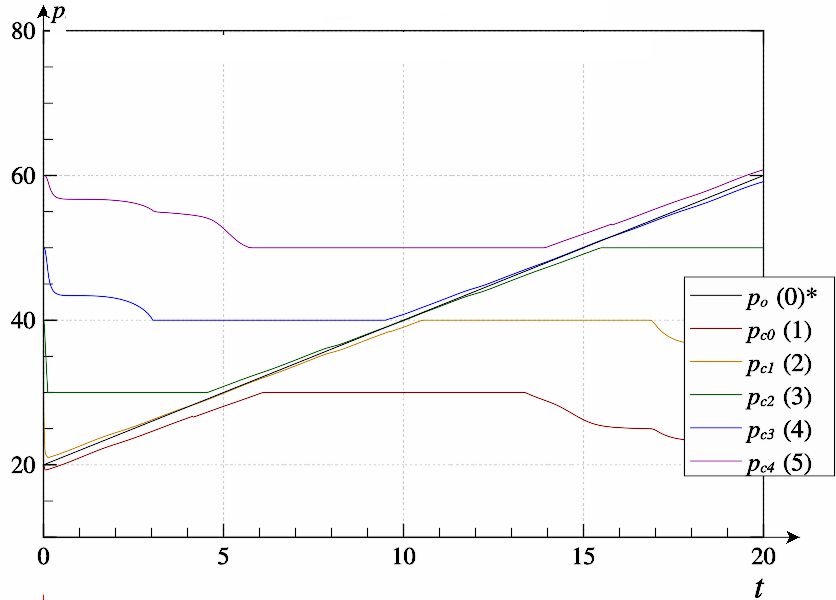
\includegraphics[width=\DDP]{../p3/p/ramp/qls-p_t_pi_ql3rlWvnAAF_ramp_xl.png}
    \\
    \parbox[t]{\DDP} {
      \caption{Рівноважні конфігурації агентів при використанні групи методів  Fq3rlovnAAF}
    \label{atu:f:qls_ramp_Fq3rlovnAAF}
  }
    \hfill
    \parbox[t]{\DDP} {
      \caption{Рівноважні конфігурації агентів при використанні групи методів ql3rlWvnAAF}
    \label{atu:f:qls_ramp_ql3rlWvnAAF}
  }
  \end{figure}


  \Xhead{Залежності $e(p_o)$}

  \begin{figure}[htb!]
    \begin{center}
      ~ \hfill
      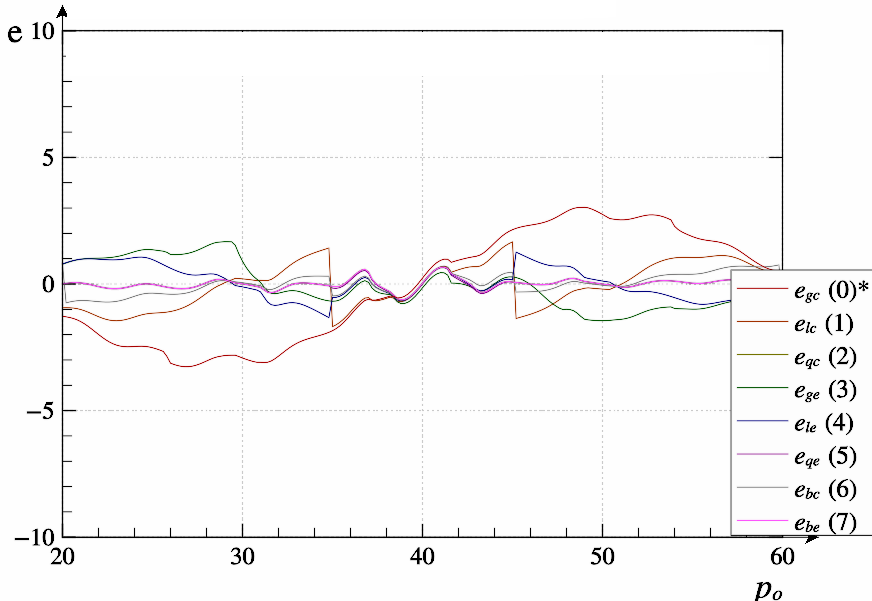
\includegraphics[width=\DDP]{../p3/p/scan/qls-p_p_e_Fq3rlFvnAAF_scan_xl.png}
      \hfill
      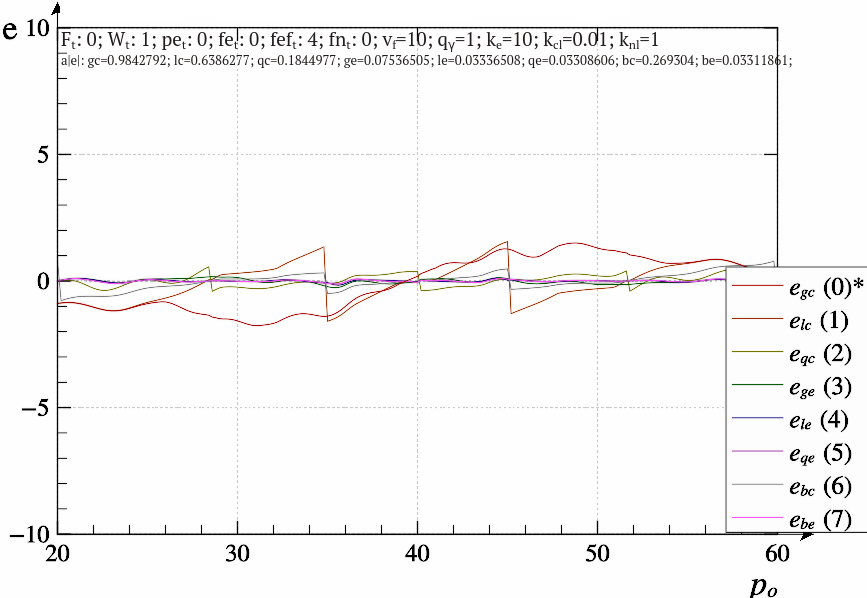
\includegraphics[width=\DDP]{../p3/p/scan/qls-p_p_e_ql3rlWvnAAW_scan_xl.png}
      \hfill ~
    \end{center}
    \parbox[t]{\DDP} {
      \caption{Залежності $e (p_o)$ для групи методів Fq3rlFvnAAF}
    \label{atu:f:Fq3rlFvnAAF_scan}
  } \hfill
    \parbox[t]{\DDP} {
      \caption{Залежності $e (p_o)$ для групи методів ql3rlWvnAAW}
    \label{atu:f:ql3rlWvnAAW_scan}
  }
  \end{figure}

\end{frame}


% -------------------------- P4 ---------------------------------------------

% -----------------------------------------------------------------------

\begin{frame}
  \frametitle{~}

  Програма ``qontrol'' була створена для моделювання динаміки
  нелінійних систем та проведення аналізу.

  Мова програмування --- C++,
  графічний інтерфейс реалізований за допомогою
  бібліотек Qt та mathGL.

  \Xhead{}
  Особливості програми ``qontrol'':

  \begin{itemize}

    \item
      Призначена для моделювання нелінійних динамічних систем як з
      використанням GUI, так і в пакетному режимі.

    \item
      Для організації об'єктної моделі використовується як можливості
      метакомпілятора ``moc'', так і власна система обробки метаданих. Це
      дозволяє як автоматично генерувати інтерфейсні елементи, так
      і встановлювати зв'язки між елементами моделі.

    \item
      Концепція ``модель --- схема --- завдання моделювання --- засоби збору і обробки інформації''
      дозволяє автоматизувати процес
      моделювання.

    \item
     Розвинені засоби представлення даних у вигляді графіків.

    \item
      У якості мови автоматизації використовується Javascript.

    \item
      Передбачено засоби взаємодії з зовнішніми програмними
      засобами. Зокрема, реалізовано взаємодію з
      вимірювально-керуючими апаратними засобами.


  \end{itemize}

  Open source, GPLv2+, \url{https://github.com/atu-guda/qontrol}


\end{frame}



% -----------------------------------------------------------------------

\begin{frame}
  \frametitle{~}
  %\framesubtitle{}

  \begin{figure}[htb!]
    \begin{center}
      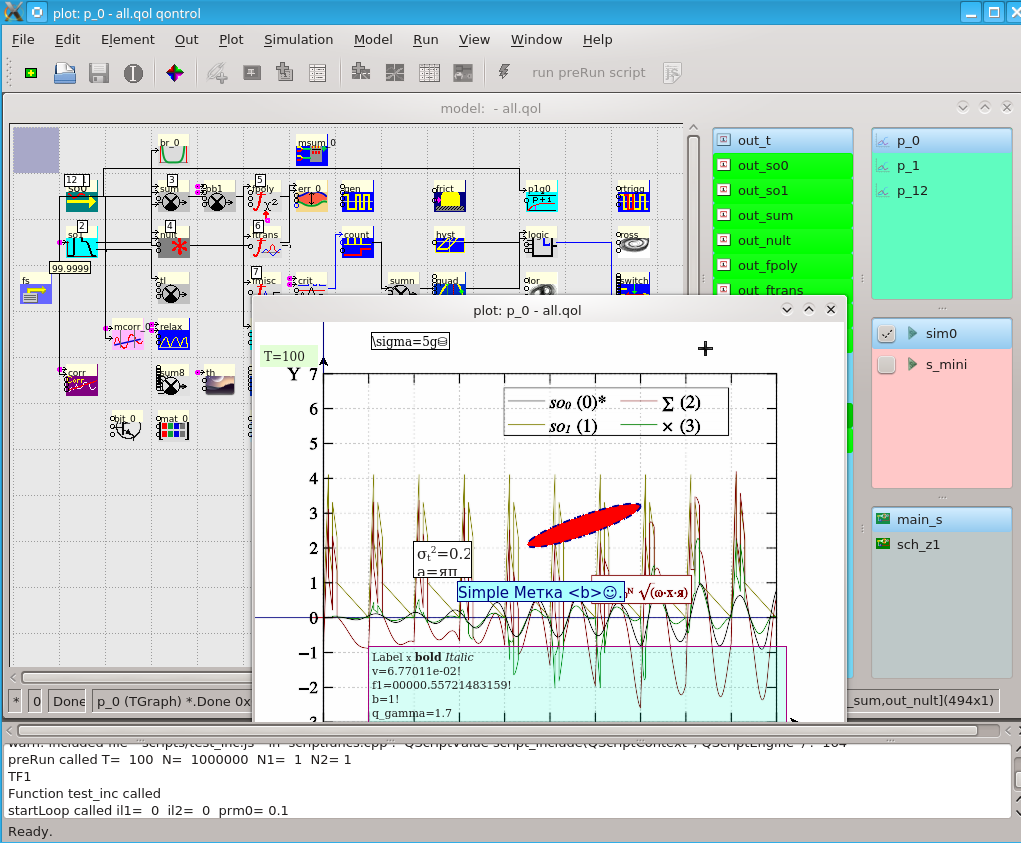
\includegraphics[width=0.82\textwidth]{../p4/p/qontrol_all.png}
    \end{center}
    \caption{Загальний вигляд інтерфейсу користувача програми ``qontrol''}
    \label{atu:f:qontrol_all}
  \end{figure}

  % \Xhead{}

  \begin{figure}[htb!]
    \begin{center}
      ~ \hfill
      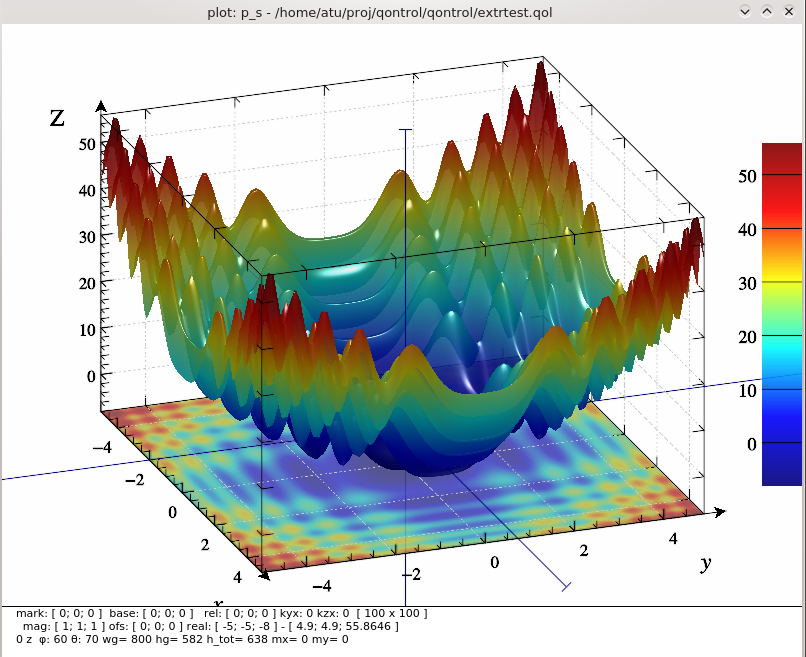
\includegraphics[width=\DDP]{../p4/p/qontrol_3d_a.png}
      \hfill
      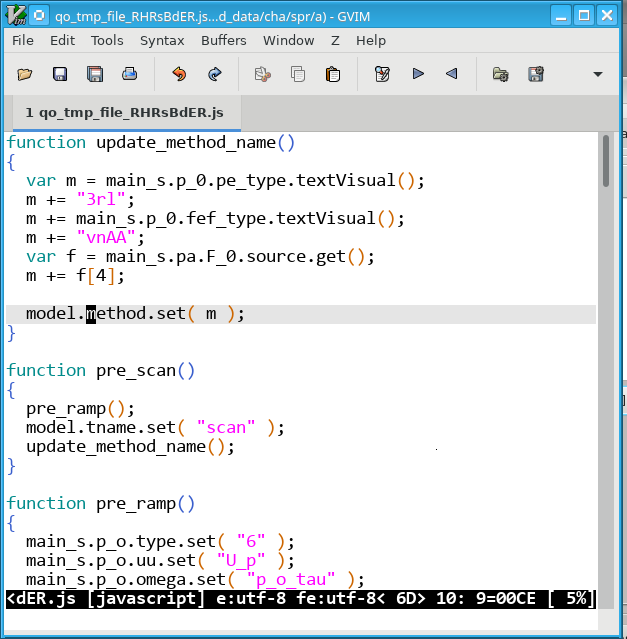
\includegraphics[width=\DDP]{../p4/p/qontrol_js.png}
      \hfill ~
    \end{center}
    \parbox[t]{\DDP} {
      \caption{Вікно, призначене для відображення графіків}
      \label{atu:f:qontrol_3d}
    } \hfill
    \parbox[t]{\DDP} {
      \caption{Приклад скриптів}
      \label{atu:f:qontrol_js}
    }
  \end{figure}


\end{frame}


% -------------------------- P5 ---------------------------------------------

% -----------------------------------------------------------------------

\begin{frame}
  \frametitle{~}

  \Xhead{Тестові системи: система Лоренца}

  \begin{equation}
    \begin{cases}
      \dot{x} = \sigma (y-x ) , \\
      \dot{y} = x (r-z) - y , \\
      \dot{z} = x y - b z .
    \end{cases}
    \label{atu:eq:lor}
  \end{equation}

  \begin{equation}
    \begin{cases}
      \pd{\vec{v}}{t} + ( \vec{v} \nabla ) \vec{v} = - \frac{\nabla p}{\rho} + \nu \Delta \vec{v} + \vec{g}, \\
      \pd{\rho}{t} + \nabla ( \rho \vec{v} ) = 0 , \\
      \pd{T}{t} +\nabla ( T \vec{v} ) = \chi \Delta T , \\
      \rho = \rho_0 \left( 1 - \gamma (T - T_0) \right) ,
    \end{cases}
    \label{atu:eq:lor_gidro}
  \end{equation}
  %
  %де
  $\Vec{v} $ --- поле швидкостей,
  $T $ --- поле температури,
  $T_0 $ і $ T_0 + \Delta T $ --- температури на верхній і нижній межі відповідно,
  $\rho $ і $ p $ --- поля щільності і тиску,
  $g $ --- прискорення вільного падіння,
  $\nu $,
  $\chi $,
  $\gamma $ --- коефіцієнти кінематичної в'язкості,
  температуропроводності і теплового розширення відповідно.

  \begin{figure}
    \PicDouble{../p5/p/cha/lor/lor0-p_xyz_r=028.png}{../p5/p/cha/lor/lor0_fft-p_f_r=028.png}
    \caption{Аттрактор (a) і спектр (b) системи Лоренца (\ref{atu:eq:lor}) в хаотичному режимі ($r = 28$)}
    \label{atu:f:lor_attractor_phase_chaos28}
  \end{figure}


\end{frame}

% -----------------------------------------------------------------------

\begin{frame}
  \frametitle{~}

  \Xhead{Система Лоренца: аналіз і вибір критеріїв}

  \begin{figure}
    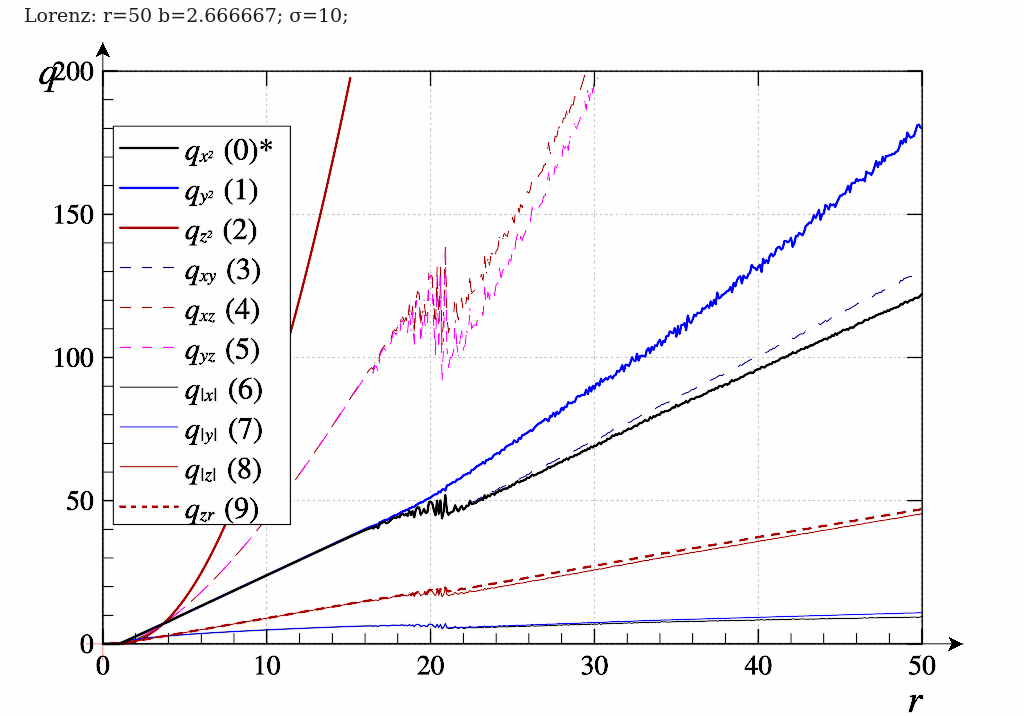
\includegraphics[width=0.7\textwidth]{../p5/p/cha/lor/lor_q-p_q_r.png}
    \caption{Розглянуті критерії для системи Лоренца}
    \label{atu:f:lor_q}
  \end{figure}

\end{frame}



% -----------------------------------------------------------------------

\begin{frame}
  \frametitle{~}

  \Xhead{Система Лоренца: залежності критеріїв для двох параметрів}

\begin{figure}[htb!]
  \PicDouble{../p5/p/cha/lor/q2d/lor_qx2_r_b.png}{../p5/p/cha/lor/q2d/lor_qy2_r_b.png}
  \PicDoubleNL{../p5/p/cha/lor/q2d/lor_qz2_r_b.png}{../p5/p/cha/lor/q2d/lor_qxmy2_r_b.png}
  \vspace{-2.7ex}
  \begin{center}
    ~ \hfill c \hfill\hfill d \hfill ~
  \end{center}
  \vspace{-1.5ex}
  \caption{Залежності $q_{x^2}(r,b)$~(a), $q_{y^2}(r,b)$~(b), $q_{z^2}(r,b)$~(c), $q_{(x-y)^2}(r,b)$~(d) для системи Лоренца}
  \label{atu:f:lor_q_r_b}
\end{figure}

  Можлива одночасна ідентифікація параметрів
  $r$ і
  $b$, за умови спільного застосування критеріїв
  $q_{x^2}$ і
  $q_{z^2}$.

\end{frame}


% -----------------------------------------------------------------------

\begin{frame}
  \frametitle{~}

  \Xhead{Система Sprott~A з додатковим параметром}

  \begin{equation}
    \begin{cases}
      \dot{x} =  c_{x_y} y, \\
      \dot{y} = -x + yz, \\
      \dot{z} =  1 - y^2.
    \end{cases}
    \label{atu:eq:spr_a}
  \end{equation}

Відмінною особливістю цієї системи є відсутність положень рівноваги, що унеможливлює
застосування багатьох відомих методів аналізу, заснованих на будь-якому
розкладі в околі точок рівноваги.

  \begin{figure}
    \PicDouble{../p5/p/cha/spr_a/sprott_a-p_xyz_cx_y=0x372.png}{../p5/p/cha/spr_a/sprott_a_f-p_f_cx_y=0x372.png}
    \caption{Аттрактор (a) та спектр (b) системи (\ref{atu:eq:spr_a}) при $c_{x_y} =0.372$}
    \label{atu:f:spr_a_p_0372}
  \end{figure}

  \begin{figure}[htb!]
    \PicDouble{../p5/p/cha/spr_a/sprott_a-p_xyz_cx_y=1x000.png}{../p5/p/cha/spr_a/sprott_a_f-p_f_cx_y=1x000.png}
    \caption{Аттрактор (a) та спектр (b) системи (\ref{atu:eq:spr_a}) при $c_{x_y} =1.0$}
    \label{atu:f:spr_a_p_1000}
  \end{figure}

\end{frame}

% -----------------------------------------------------------------------

\begin{frame}
  \frametitle{~}

  \Xhead{}

\begin{figure}
  \begin{center}
    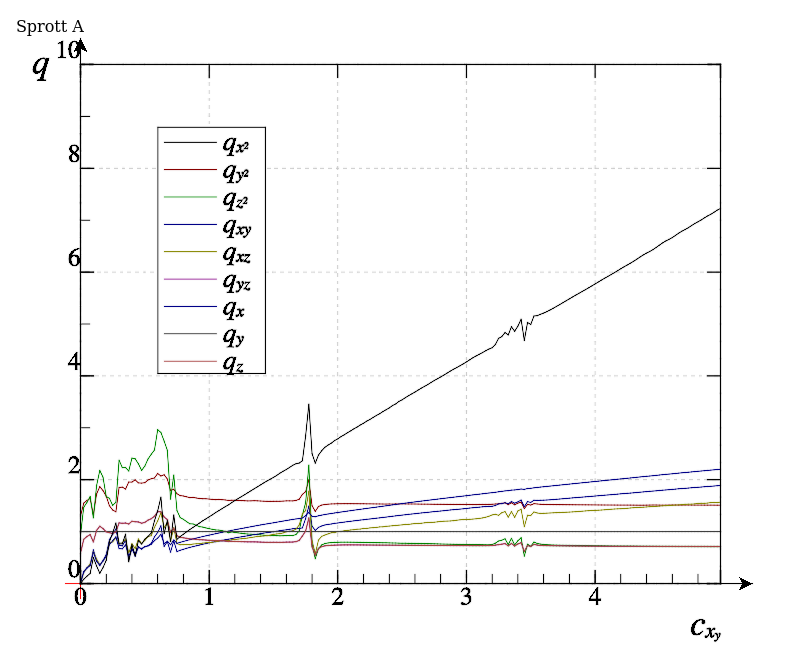
\includegraphics[width=0.60\textwidth]{../p5/p/cha/spr_a/sprott_a_q-p_c_x_y.png}
  \end{center}
  \caption{Залежності $q_{*}(c_{x_y})$ для системи (\ref{atu:eq:spr_a})}
  \label{atu:f:spr_a_q}
\end{figure}


\end{frame}





% -------------------------- P6 ---------------------------------------------


% -----------------------------------------------------------------------

\begin{frame}
  \frametitle{~}

  \Xhead{}

  Програмно-апаратна складова комплексу реалізована на
  мікроконтролерах STM32 (ARM Cortex M4F). Використовувалася як власна
  розробка за базі STM32F407VE, так і отладочная плата на STM32F746ZI +
  допоміжні елементи.

  \begin{figure}[ht!]
    \centerline{\includegraphics[width=90\TW]{../p6/p/colp_stand.png} }
    \caption{Апаратно-програмний комплекс при роботі з генератором Колпітца}
    \label{atu:colp_stand}
  \end{figure}



\end{frame}


% -----------------------------------------------------------------------

\begin{frame}
  \frametitle{~}
  %\framesubtitle{}
  \Xhead{Моделювання та ідентифікація фізичної системи пов'язаних релаксаційних генераторів}

  \begin{figure}
    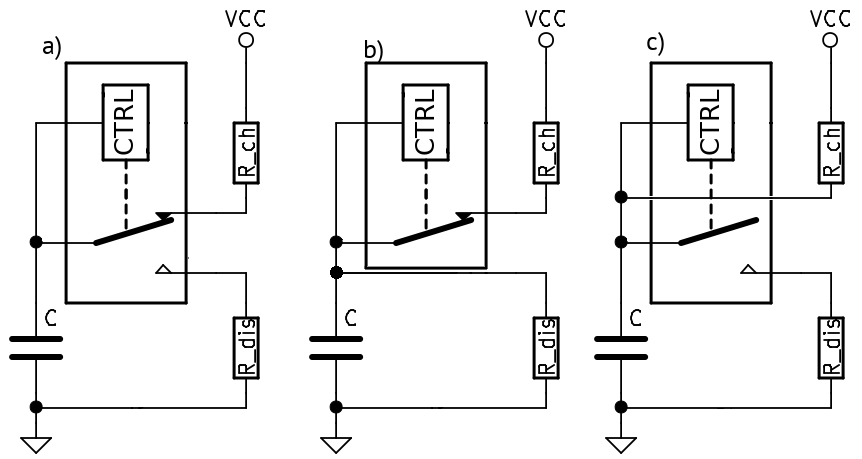
\includegraphics[width=0.60\textwidth]{../p7/p/relax_types.png}
    \caption{Умовні схеми релаксаційних генераторів}
  \end{figure}

\begin{equation}
  C \od{V_c}{t}
  =
  \frac{V\Tidx{cc} - V\Tidx{c}}{R\Tidx{ch}}
  - \frac{V\Tidx{c}}{R\Tidx{dis}} \cdot \mathrm{On}().
  \label{atu:eq:relax0}
\end{equation}

  \begin{figure}
    \centerline{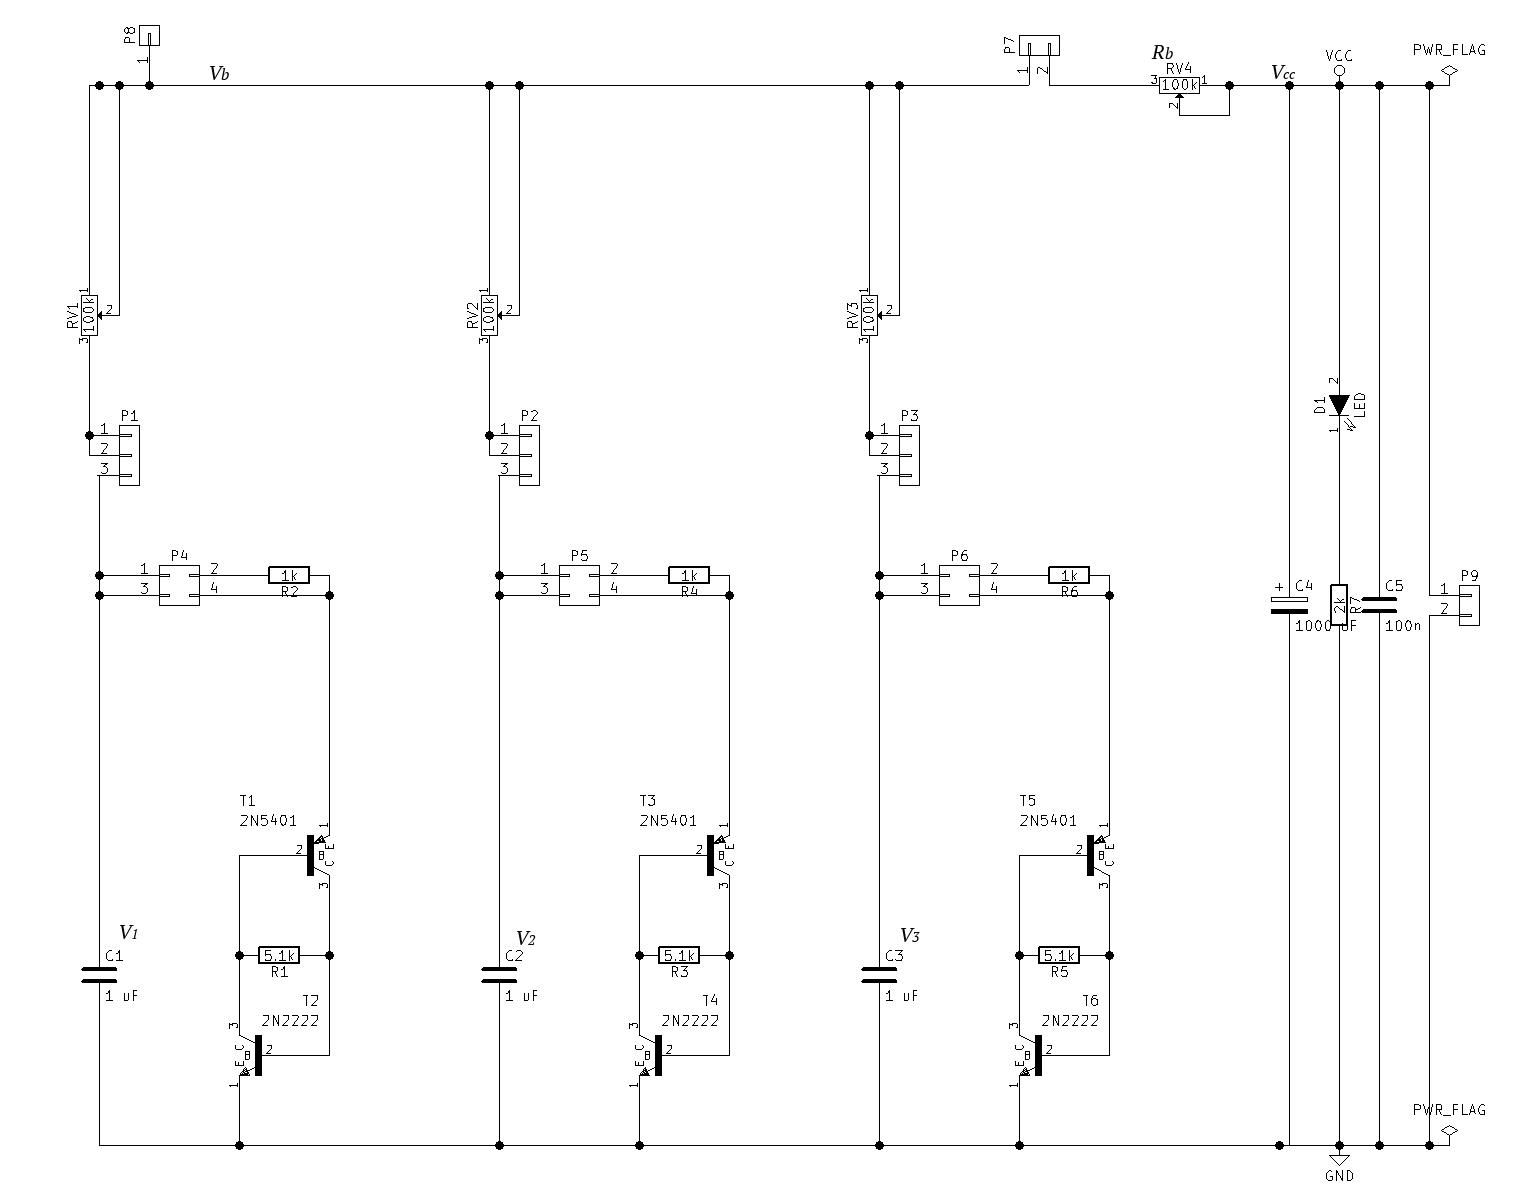
\includegraphics[width=0.86\textwidth]{../p7/p/relax3d_schem.png} }
    \caption{Електрична схема \RelaxBjtIi}
  \end{figure}


\end{frame}


% -----------------------------------------------------------------------

\begin{frame}
  \frametitle{~}
  %\framesubtitle{}

  \Xhead{}

  \begin{figure}
    \PicDoubleS{../p7/p/relax3d_f_02.png}{../p7/p/relax3d_v1v2v3_02.png}
    \caption{Спектр $V_b(t)$~(a), і аттрактор~(b) для системи ``relax3d'' при $R_b = \SI{5.0}{\kilo \ohm} $}
    \label{atu:f:relax3d_f_02}
  \end{figure}

  \begin{figure}
    \PicDoubleS{../p7/p/relax3d_f_08.png}{../p7/p/relax3d_v1v2v3_08.png}
    \caption{Спектр $V_b(t)$~(a), і аттрактор~(b) для системи ``relax3d'' при $ R_b = \SI{34.0}{\kilo\ohm} $}
    \label{atu:f:relax3d_f_08}
  \end{figure}

  \begin{figure}
    \PicDoubleS{../p7/p/relax3d_f_09.png}{../p7/p/relax3d_v1v2v3_09.png}
    \caption{Спектр $V_b(t)$~(a), и аттрактор~(b) для системи ``relax3d'' при $R_b=\SI{36.0}{\kilo\ohm}$ }
    \label{atu:f:relax3d_f_09}
  \end{figure}

\end{frame}


% -----------------------------------------------------------------------

\begin{frame}
  \frametitle{~}
  %\framesubtitle{}

  \Xhead{Модель систем з трьох пов'язаних релаксаційних генераторів}

  \begin{equation}
  \begin{cases}
    V_b = V_{cc} - R_b ( I_1 + I_2 + I_3 ), \\
      C_1 \dot{V}_1 = \frac{V_b-V_1}{R_{v1}} - \frac{V_1}{R_1} \mathrm{On}_1() - I_{1,\mathrm{leak}}(V_1), \\
      C_2 \dot{V}_2 = \frac{V_b-V_2}{R_{v2}} - \frac{V_2}{R_2} \mathrm{On}_2() - I_{2,\mathrm{leak}}(V_2), \\
      C_3 \dot{V}_3 = \frac{V_b-V_3}{R_{v3}} - \frac{V_3}{R_3} \mathrm{On}_3() - I_{3,\mathrm{leak}}(V_3), \\
      I_i = \frac{V_b-V_i}{R_{vi}}.
  \end{cases}.
    \label{atu:eq:relax3}
\end{equation}
%
де: \\
$R_b $ --- опір в ланцюзі живлення (ідентифікований параметр),
$C_i $ --- ємності кожного з релаксаційних генераторів,
$R_{vi} $ --- опори зарядки релаксаційних генераторів,
$R_{ i} $ --- опори зарядки релаксаційних генераторів,
$I_{i, \mathrm{leak}} $ --- струми витоку.


\end{frame}


% -----------------------------------------------------------------------

\begin{frame}
  \frametitle{~}
  %\framesubtitle{}

  \Xhead{Критерії ідентифікації для системи ``relax3d''}

\begin{equation}
  q_{sv} = \overline{V_1+V_2+V_3} .
  \label{atu:eq:q_sv_relax}
\end{equation}
%
\begin{equation}
  q_{vb} = \overline{V_b} .
  \label{atu:eq:q_vb_relax}
\end{equation}
%
\begin{equation}
  q_{hv} = \frac{1}{\overline{V_b}} .
  \label{atu:eq:q_hb_relax}
\end{equation}
%
\begin{equation}
  q_{rv} = \frac{\overline{V_1+V_2+V_3}}{\overline{V_b}}.
  \label{atu:eq:q_rv_relax}
\end{equation}

  \begin{figure}
    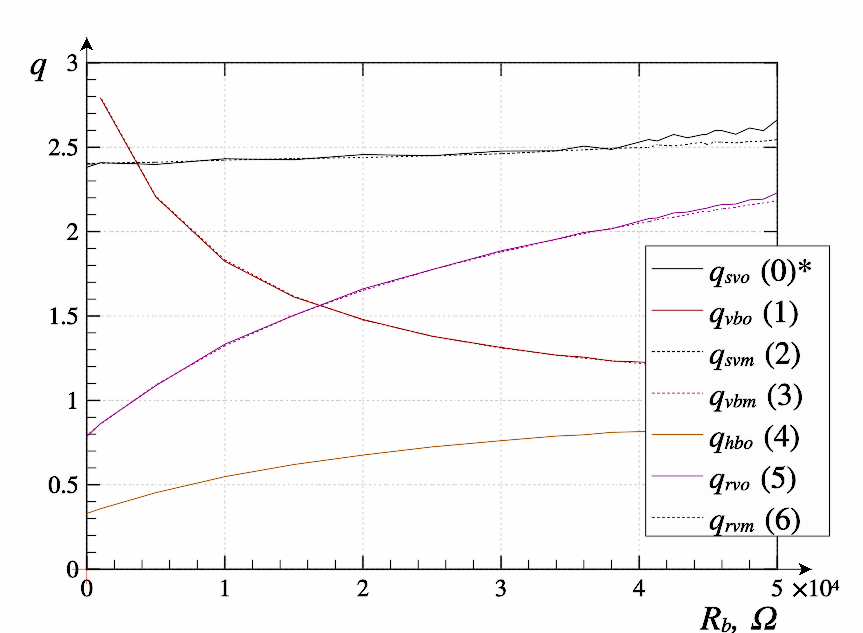
\includegraphics[width=0.7\textwidth]{../p7/p/relax3d_read_q-p_q1.png}
    \caption{Залежності для розглянутих критеріїв ідентифікації для системи релаксаційних генераторів на парі компліментарних транзисторів}
  \end{figure}


\end{frame}


% -----------------------------------------------------------------------

\begin{frame}
  \frametitle{~}
  %\framesubtitle{}

  \Xhead{}

  \begin{figure}
    \PicDouble{../p7/p/relax3ds_read_id2_0-p_p.png}{../p7/p/relax3ds_read_id2_0-p_pp.png}
    \caption{Процес ідентифікації системи ``relax3ds'' групою методів ``Fq3zlovnAAF'': динаміка агентів~(a) та $p_\mathrm{id}$~(b)}
  \end{figure}

  \begin{figure}
    \PicDoubleNL{../p7/p/relax3ds_read_id2_prm_0-p_a_q.png}{../p7/p/relax3ds_read_id2_prm_0-p_q_gamma.png}
    \TextDouble{\caption{Залежності $\overline{e}_{r *}(a_q)$ при ідентифікації системи ``relax3ds''}}{\caption{Залежності $ \overline{e}_{r *} (q_\gamma) $ при ідентифікації системи ``relax3ds''}}
  \end{figure}


\end{frame}

% ----------------------------- FINAL ------------------------------------------

\begin{frame}
  \frametitle{Наукова новизна}
  %\framesubtitle{}

  \Xhead{Наукова новизна}

  \noindent
  \textbf{Вперше:}
  %
  \begin{itemize}

    \item
      створено критерії ідентифікації нелінійних динамічних систем,
      які, на відміну від тих, що існують, дозволяють оцінити їх стан та
      хаотичну динаміку, а також дають підстави для створення ефективних алгоритмів
      настроювання параметрів моделей систем ідентифікації;

    \item
      створено методи ідентифікації на підставі
      адаптивно-пошукової парадигми з використанням ансамблю пошукових агентів,
      які взаємодіють проміж собою, які на відміну від методів, що використовують
      одну модель або пару моделей, значно підвищують швидкість пошуку та
      здатні за мінімальний час  перелаштовуватися при різкій зміні параметрів, а на
      відміну від ройових алгоритмів нові методи потребують значно меншої
      кількості моделей та забезпечують певні гарантії пошуку;

    \item
      створено нову класифікацію систем ідентифікації динамічних систем,
      яка, як вбирає у себе методи, що існують, так і дозволяє
      створювати нові методи ідентифікації за рахунок
      комбінування їх складових частин;

    \item
      визначено, що системи з сухим тертям з точки зору задачі ідентифікації
      при певних  умовах функціонування
      мають властивості, що поєднують їх з системами хаотичної динаміки, тобто існує
      суттєва залежність від початкових
      умов та характерний вид атрактору;

    \item
      запропоновано модель системи хаотичної динаміки
      з використанням зв'язаних релаксаційних генераторів,
      яка відрізняється від існуючих відсутністю індуктивних компонентів,
      працездатністю при малих напругах та можливістю
      керування частотним діапазоном у широкому інтервалі,
      що сприяє процесу аналізу хаотичної динаміки
      фізичного об'єкту, перевірці адекватності математичної моделі
      та властивостей системи ідентифікації.
  \end{itemize}


\end{frame}




% -----------------------------------------------------------------------

\begin{frame}
  \frametitle{Практическая ценность}
  %\framesubtitle{}

  \noindent
  \textbf{ Набуло подальший розвиток:}
  \begin{itemize}

    \item
      методи оцінювання якості ідентифікації,
      які на відміну від тих, що існують,
      враховують використання множини агентів;

    \item
      підходи до адаптації параметрів систем
      ансамблевої ідентифікації, які придатні використовувати поточну
      інформацію від ансамблю синергірованих моделей та коригувати глобальні
      параметри пошуку в умовах апріорної та поточної невизначеності;

    \item
      модель генератора Колпітца, яка враховує
      більшу кількість нелінійних ефектів,
      що забезпечує більш адекватні результати процесу
      ідентифікації її параметрів запропонованими методами;
  \end{itemize}


\textbf{Практичне значення одержаних результатів.}
Розроблені методи ідентифікації було використано
при проектуванні, створенні, налаштовуванні параметрів
стенду дослідження вібраційного та акустичного впливу.
Аналіз результатів даних з цього стенду
дав можливість вказати необхідні нелінійні властивості системи
та діапазон параметрів, які у сукупності
забезпечують широкосмуговий спектр коливань.

Створене програмне середовище для моделювання нелінійних динамічних систем
використовується при проведенні практичних робіт по дисциплінам
``Моделювання систем'',
``Сучасні системи управління'' на кафедрі інформаційних технологій
і систем Національної металургійної академії України.

\end{frame}





% -----------------------------------------------------------------------

\begin{frame}
  \frametitle{Друковані роботи та апробація}
  %\framesubtitle{}

  \Xhead{Друковані роботи та апробація}

За темою дисертаційної роботи опубліковано
50 наукових праць. Основний зміст і результати досліджень
викладено у 36 друкованих працях у наукових фахових виданнях, які
рекомендовано Міністерством освіти і науки України,
29 --- включено до інших міжнародних наукометричних баз,
у тому числі 1 --- включено до бази Web of Science,
13 робіт опубліковано у збірниках наукових праць та матеріалах конференцій.

\smallskip

%{\scriptsize
Основные положения диссертационной работы докладывались на
научно-практических конференциях:
``Інформатика та системні науки'' (ІСН-2011) Полтава--2011,
``Интеллектуальные системы принятия решений и проблемы вычислительного интеллекта'' (ISDMCI) Херсон--2011,
``Информационные технологии в управлении сложными системами'' Днепропетровск--2011,
``Автоматизация: проблемы, идеи, решения'' Севастополь--2011,
``Интеллектуальные системы принятия решений и проблемы вычислительного интеллекта'' (ISDMCI) Херсон--2012,
``Автоматизация: проблемы, идеи, решения'' Севастополь--2012,
``Интеллектуальные системы принятия решений и проблемы вычислительного интеллекта'' (ISDMCI) Херсон--2013,
``Автоматизация: проблемы, идеи, решения'' Севастополь--2013,
``Интеллектуальные системы принятия решений и проблемы вычислительного интеллекта'' (ISDMCI) Херсон--2014,
``Интеллектуальные системы принятия решений и проблемы вычислительного интеллекта'' (ISDMCI) Херсон--2015,
``Computer Sciences and Information Technologies'' (CSIT) Lviv--2015 (Scopus),
``Интеллектуальные системы принятия решений и проблемы вычислительного интеллекта'' (ISDMCI) Херсон--2016,
``Data Stream Mining and Processing'' DSMP Lviv--2016 (Scopus,Web of Science).
%} % scriptsize

\end{frame}




% -----------------------------------------------------------------------

\begin{frame}
  \frametitle{Висновки}
  %\framesubtitle{}

  \Xhead{Висновки}

У роботі вирішена науково-технічна проблема ідентифікації параметрів складних технічних
систем у режимі хаотичної динаміки
з метою забезпечення їх керованої поведінки. При цьому:

\begin{itemize}

  \item
    створено нові критерії ідентифікації, які, на відміну від тих, що
    існують, придатні для аналізу стану та динаміки
    хаотичних систем, що створило фізично зумовлене обґрунтування працездатності систем
    ідентифікації;

  \item
    створено новий клас систем ідентифікації у межах
    адаптивно-пошуковой парадигми,
    які, за рахунок використання колективної динаміки
    ансамблю пошукових агентів, забезпечують
    кращу швидкість ідентифікації без істотного впливу на похибку ідентифікації;

  \item
    проведена перевірка працездатності запропонованих методів
    на прикладах як відомих систем хаотичної динаміки,
    так і на прикладах декількох інших динамічних систем (модельних та фізичних),
    які проявляють складну та хаотичну динаміку;

  \item
   визначено, що системи з сухим тертям з точки зору задачі ідентифікації
   при певних  умовах функціонування
   мають властивості, що поєднують їх з системами хаотичної динаміки;

 \item
  створено програмне забезпечення, придатне для моделювання як систем
  хаотичної динаміки, так і систем мультиагентної ідентифікації;

  \item
  проведено як комп'ютерне моделювання процесів ідентифікації систем
  хаотичної динаміки, так і фізичне моделювання таких, що підтверджує адекватність
  побудованих моделей.


\end{itemize}

\end{frame}



% -----------------------------------------------------------------------
%
% \begin{frame}
%   \frametitle{Выводы 2}
%   %\framesubtitle{}
%
%
% \end{frame}



\end{document}

